\documentclass[../main.tex]{subfiles}
\begin{document}
\graphicspath{{figures/}{task3/figures/}}

\subsection{Task 3: Player Monthly Spending Prediction (NMAE)}
\label{sec:t3}

\subsubsection{Problem and Data}

Task 3 asks for the amount, in Thai baht, that each player will spend in the next 30 days (\feat{spending_30d}). The score is the \textbf{normalised MAE score}
\[
\text{NMAE score}=\frac{1}{1+\mathrm{MAE}/\overline{|y|}}=\frac{1}{1+\sum_i|y_i-\hat y_i|\,/\sum_i y_i},
\]
which lies in $(0,1]$ and rises as the error falls. Predicting zero for everyone scores exactly 0.5. A leaderboard probe supports this reading: when we replaced our Task~3 predictions by zeros, the public score fell by 0.0590, which is 0.2 times $(0.795-0.5)$. This is what a score of 0.795 for our model and a task weight of 0.2 predict, in agreement with cross-validation.

The training set has 104{,}000 rows and the test set 25{,}889. Each row has 32 features: activity (friends, sessions, login recency, playtime, achievements), money (\feat{historical_spending}, \feat{prev_month_spending}, \feat{total_transactions}, \feat{avg_transaction_value}, \feat{discount_rate_used}, \feat{purchase_frequency}), and account traits (\feat{vip_status}, \feat{is_premium_member}, \feat{games_played}, \feat{segment}, month). About 5.8\% of the money columns and 5.7\% of \feat{segment} are missing.

\subsubsection{EDA Findings}
\label{sec:t3-eda}

The target decides the model, so we studied it first: how many players spend nothing, who produces the money, which columns are linked exactly, and how well last month's spending predicts this month's.

\paragraph{A zero-inflated, heavy-tailed target.} Figure~\ref{fig:t3-target} shows how many players pay and how much.

\begin{figure}[H]
\centering
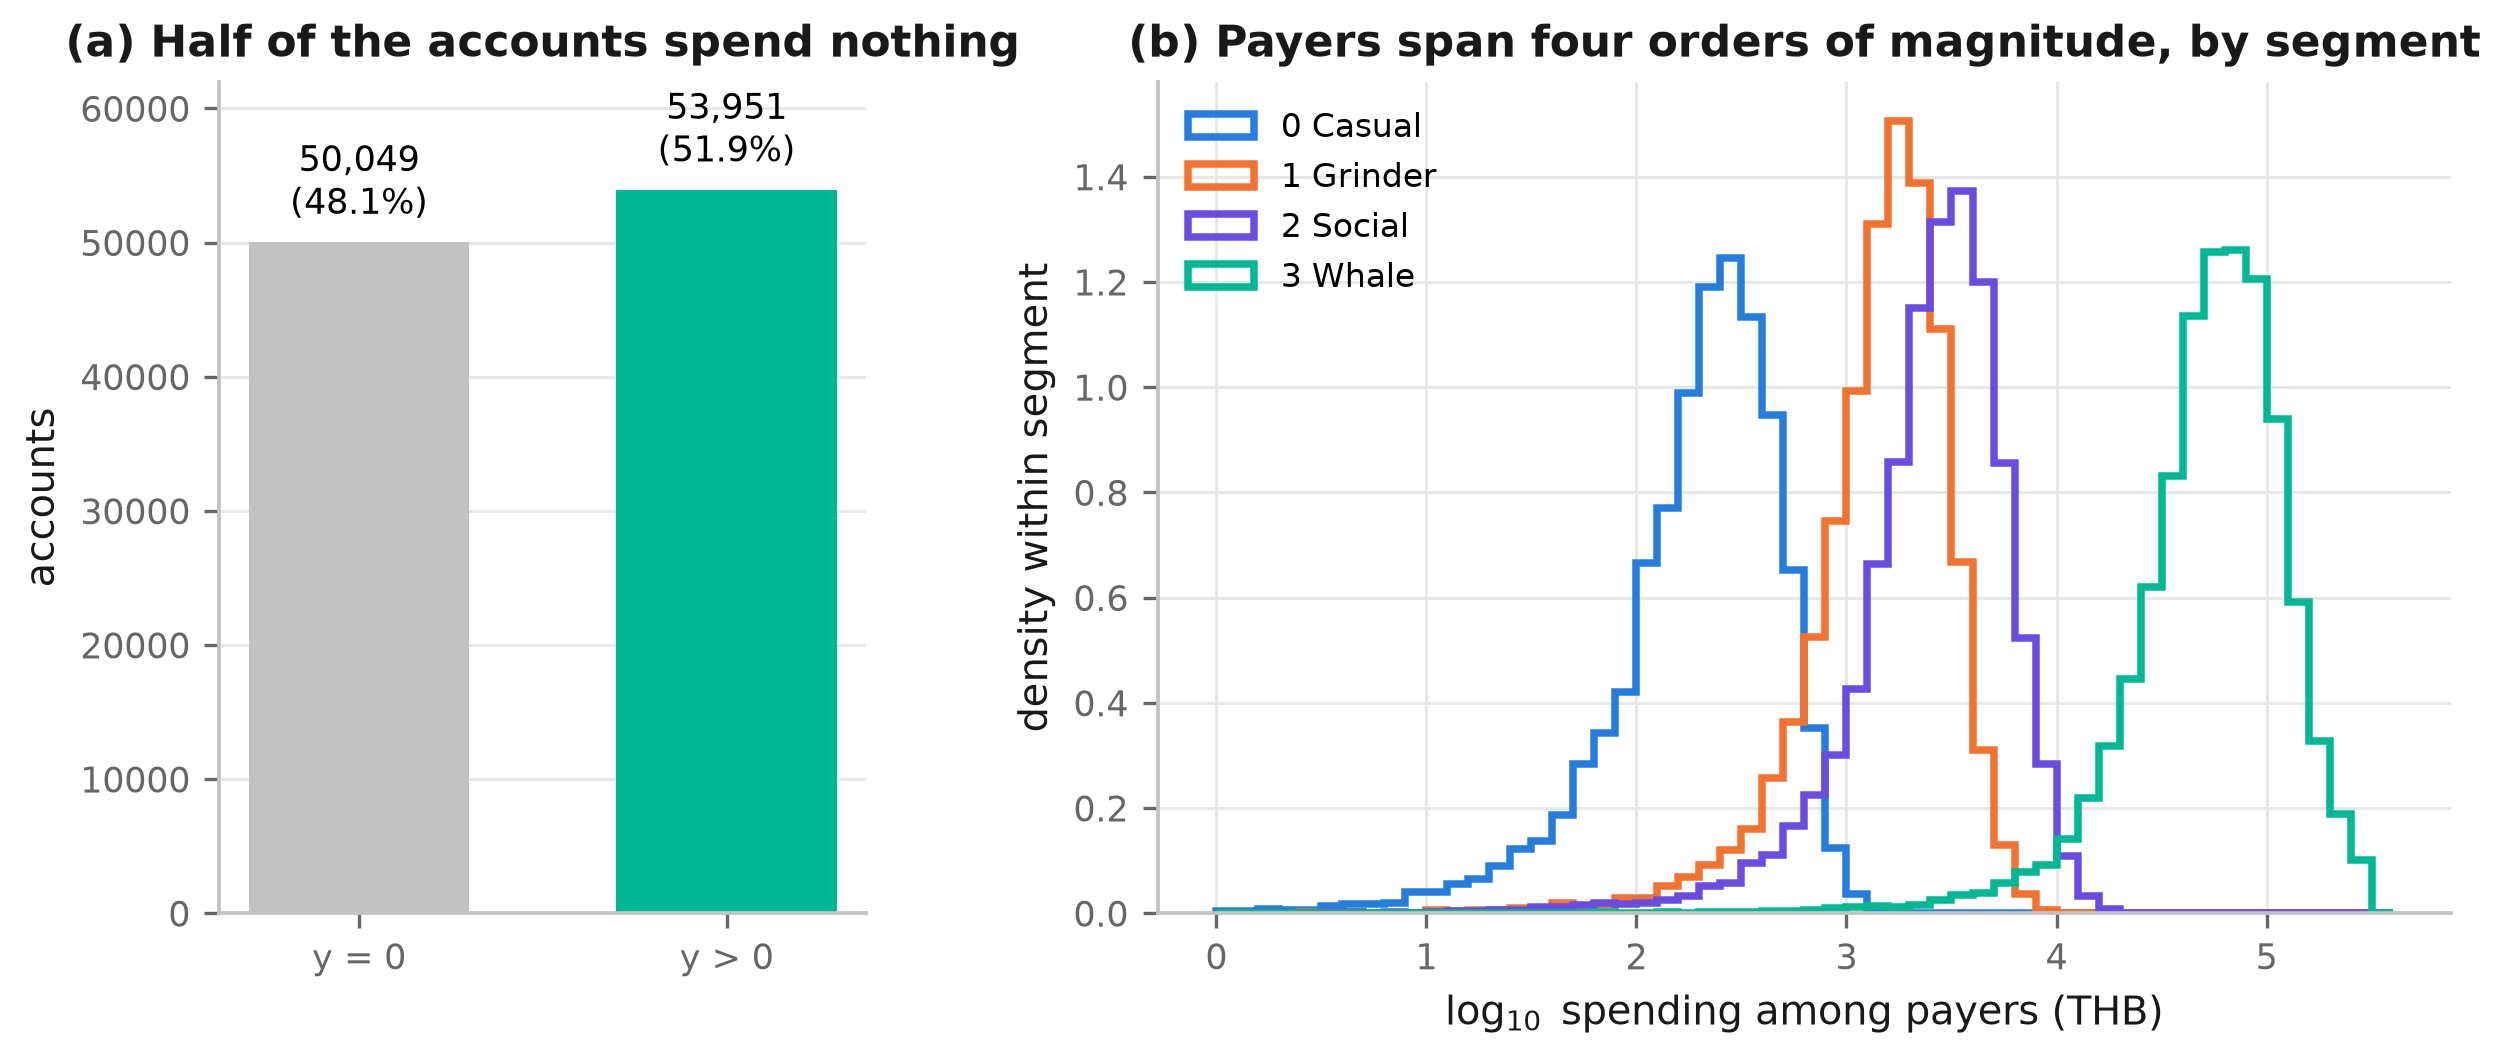
\includegraphics[width=\linewidth,height=0.33\textheight,keepaspectratio]{fig_t3_target.png}
\caption{(a) 48.1\% of the training accounts spend exactly zero. (b) Distribution of $\log_{10}$ spending among payers, one curve per segment; each segment sits at a different level.}
\label{fig:t3-target}
\end{figure}

\emph{What we see.} 50{,}049 of 104{,}000 accounts (48.1\%) spend nothing. Among payers the median is 2{,}314 THB, the mean is 20{,}235 THB and the maximum is 300{,}000, which looks like a cap. The four segments are separated almost cleanly on the log scale: payer medians are 229, 1{,}627, 2{,}855 and 58{,}618 THB for segments 0 to 3. A single regression curve would therefore have to model a spike at zero and a spread over four orders of magnitude at the same time. \emph{What we decided.} Use a two-stage \emph{hurdle} model: one model for whether a player pays and one for how much, and work on the logarithm of the amount.

\paragraph{Who produces the money.} Figure~\ref{fig:t3-whales} compares shares of accounts and of spending by segment.

\begin{figure}[H]
\centering
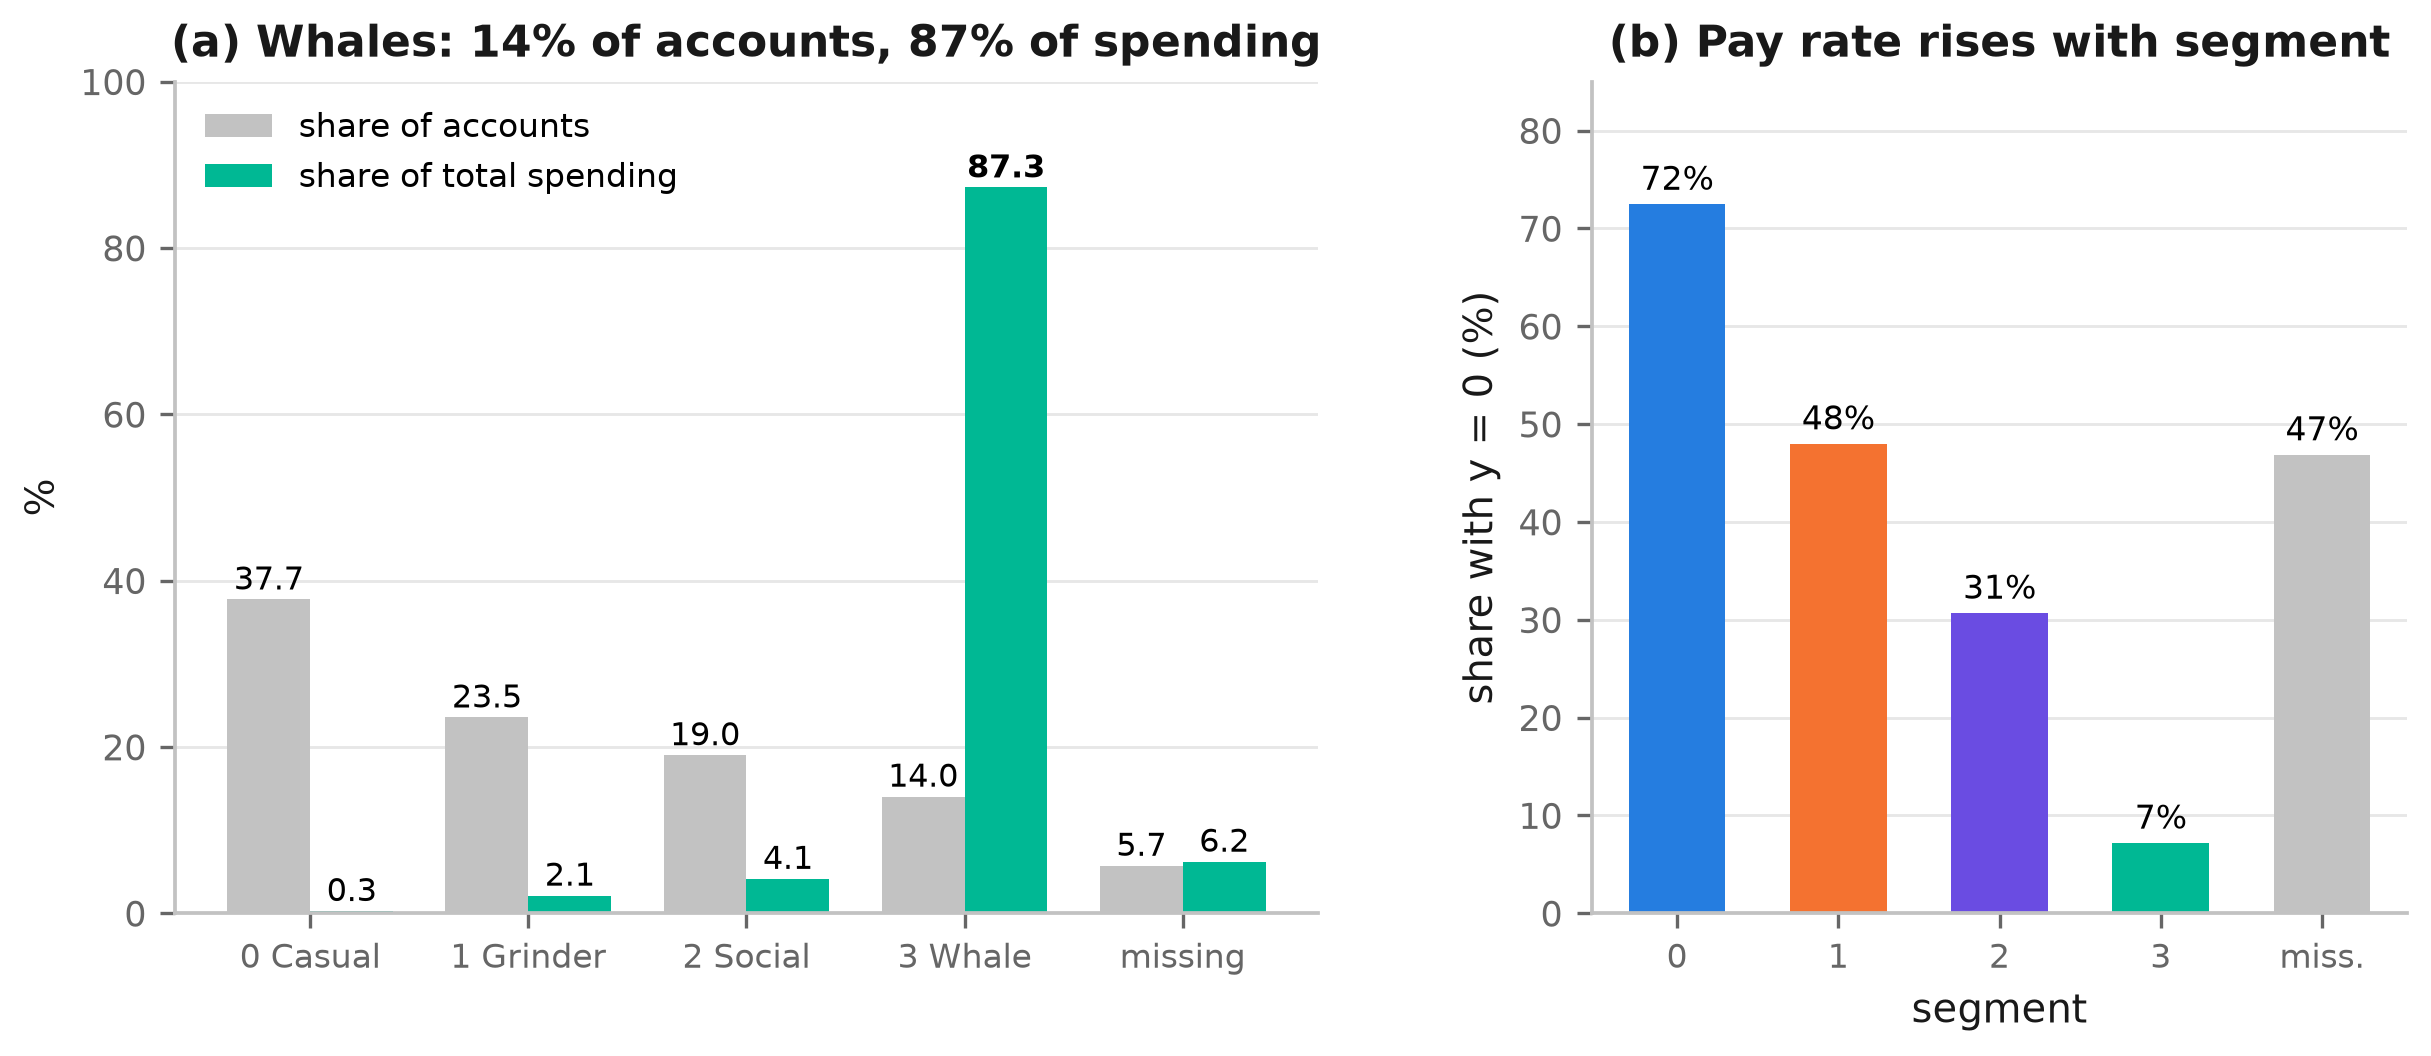
\includegraphics[width=\linewidth,height=0.33\textheight,keepaspectratio]{fig_t3_whales.png}
\caption{(a) Share of accounts and of total spending by segment; ``missing'' marks the 5.7\% of rows without a segment. (b) Share of players with zero spending by segment.}
\label{fig:t3-whales}
\end{figure}

\emph{What we see.} Segment 3 (whales) is 14.0\% of the accounts and 87.3\% of all money, with a mean of 65{,}358 THB against 74 THB for segment 0. Only 7.1\% of whales spend nothing, against 72.4\% of Casual players. Rows with a missing segment still carry 6.2\% of the spending. Because MAE weighs a baht equally everywhere, the whales dominate the metric. \emph{What we decided.} Segment is a key input, so we impute the missing segment with a classifier trained on the training rows, and we add the probability of being a whale as a feature.

\paragraph{Exact relations among the money columns.} We tested whether the columns \feat{historical_spending}, \feat{total_transactions}, \feat{avg_transaction_value}, \feat{purchases_on_discount} and \feat{discount_rate_used} are linked by exact identities (Figure~\ref{fig:t3-identities}).

\begin{figure}[H]
\centering
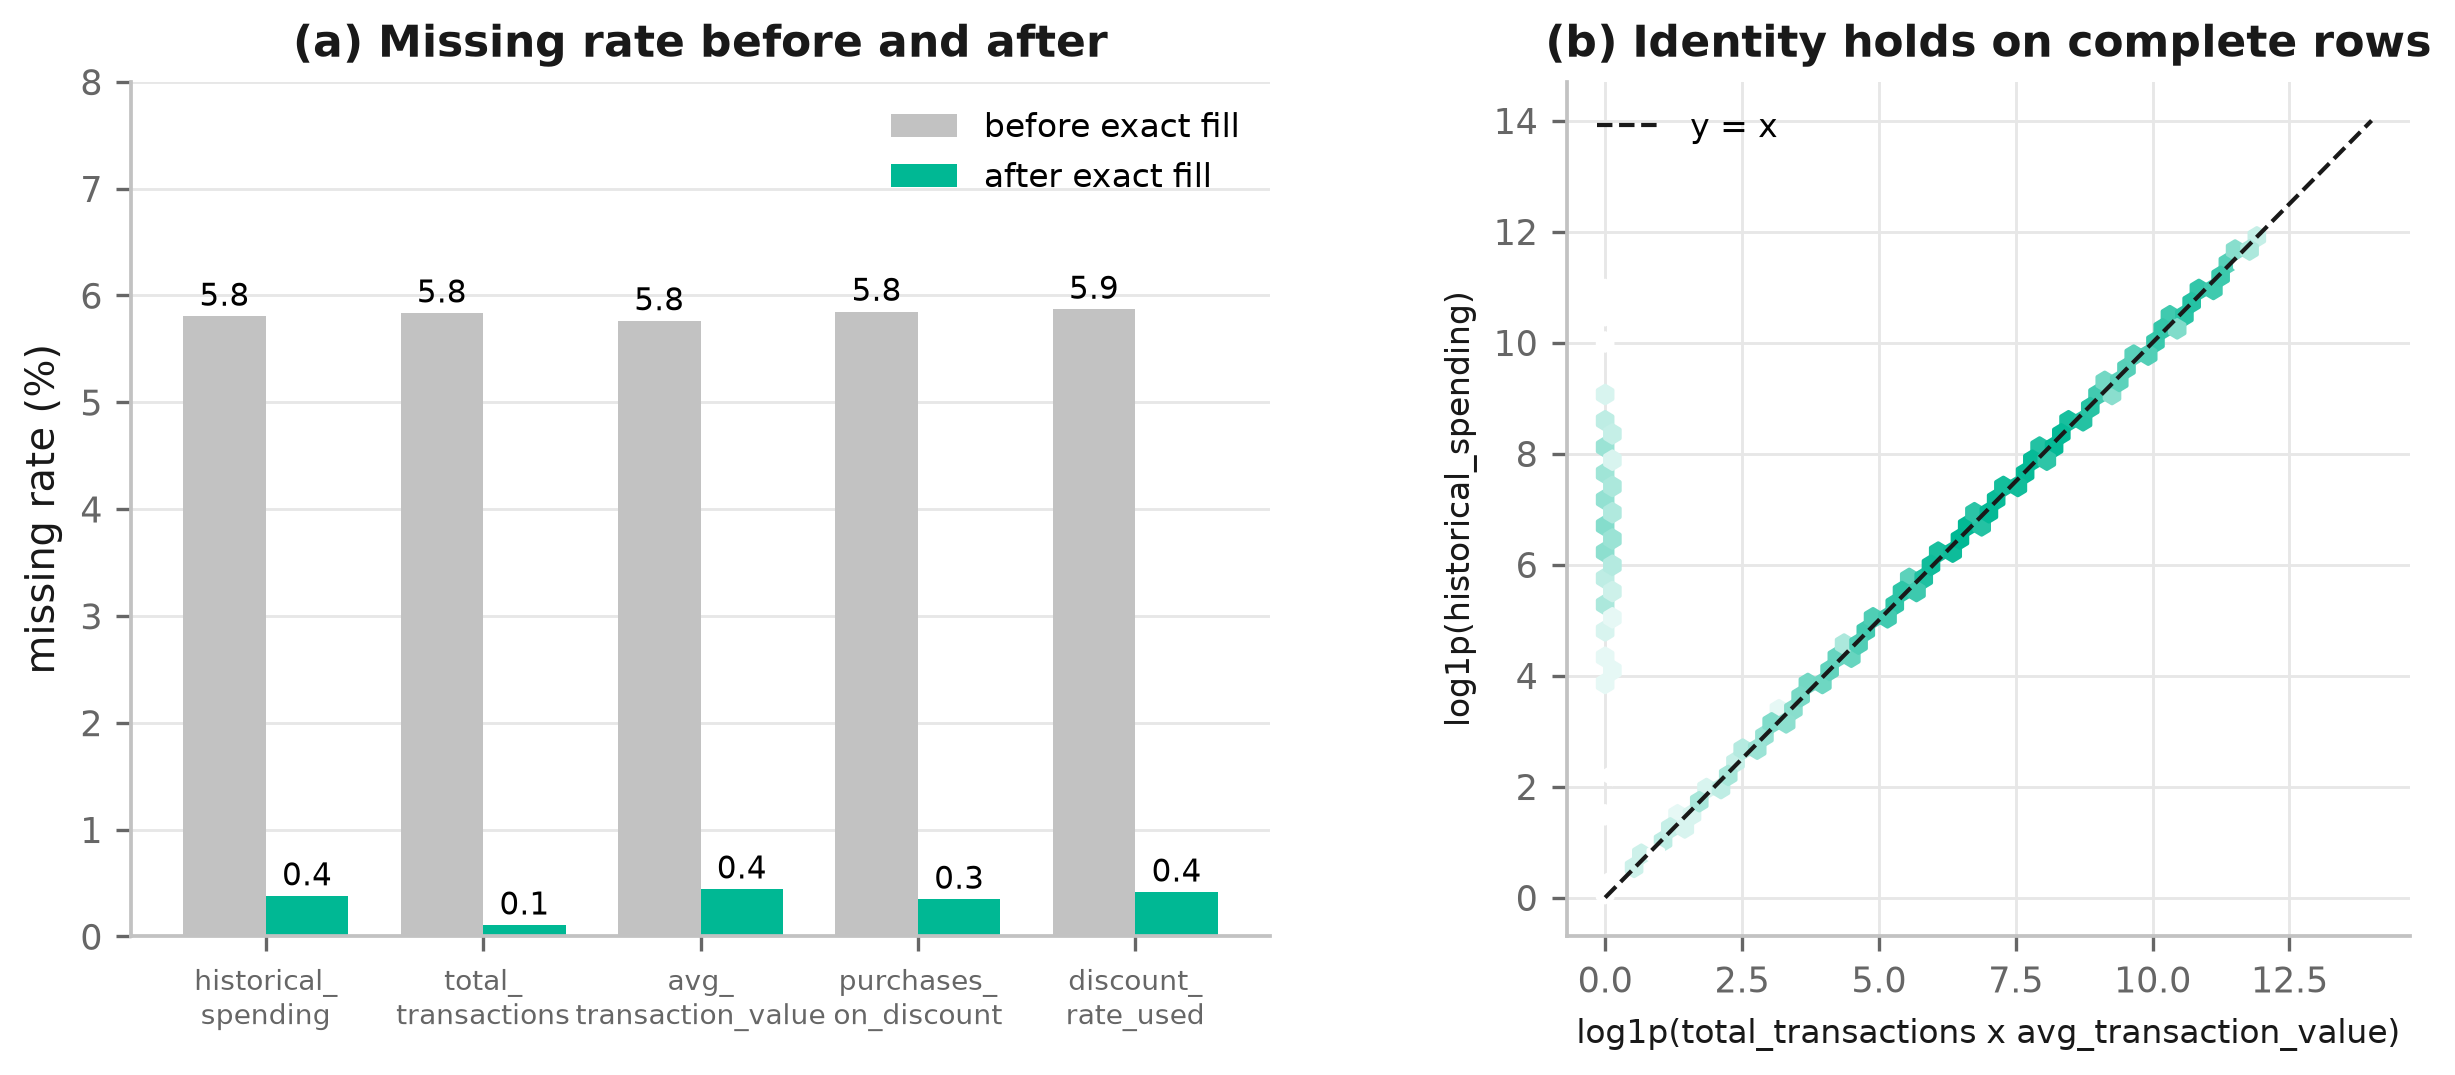
\includegraphics[width=\linewidth,height=0.33\textheight,keepaspectratio]{fig_t3_identities.png}
\caption{(a) Missing rate of the five money columns before and after the exact fill. (b) On 20{,}000 complete rows, \texttt{historical\_spending} lies on the line $y=x$ against \texttt{total\_transactions}~$\times$~\texttt{avg\_transaction\_value}.}
\label{fig:t3-identities}
\end{figure}

\emph{What we see.} $\texttt{historical\_spending}=\texttt{total\_transactions}\times\texttt{avg\_transaction\_value}$ holds exactly on 99.0\% of complete rows and $\texttt{purchases\_on\_discount}=\texttt{total\_transactions}\times\texttt{discount\_rate\_used}$ on 100\%; the median error is zero. Each column is missing in about 5.8\% of the rows, so one missing value can often be recovered from the other two. \emph{What we decided.} Fill missing values with the exact identities before any modelling. Missing rates fall from 5.8\% to between 0.1\% and 0.44\%, and the fill uses no model, hence no leakage.

\paragraph{Last month predicts this month.} Figure~\ref{fig:t3-offset} relates \feat{prev_month_spending} to the target for payers.

\begin{figure}[H]
\centering
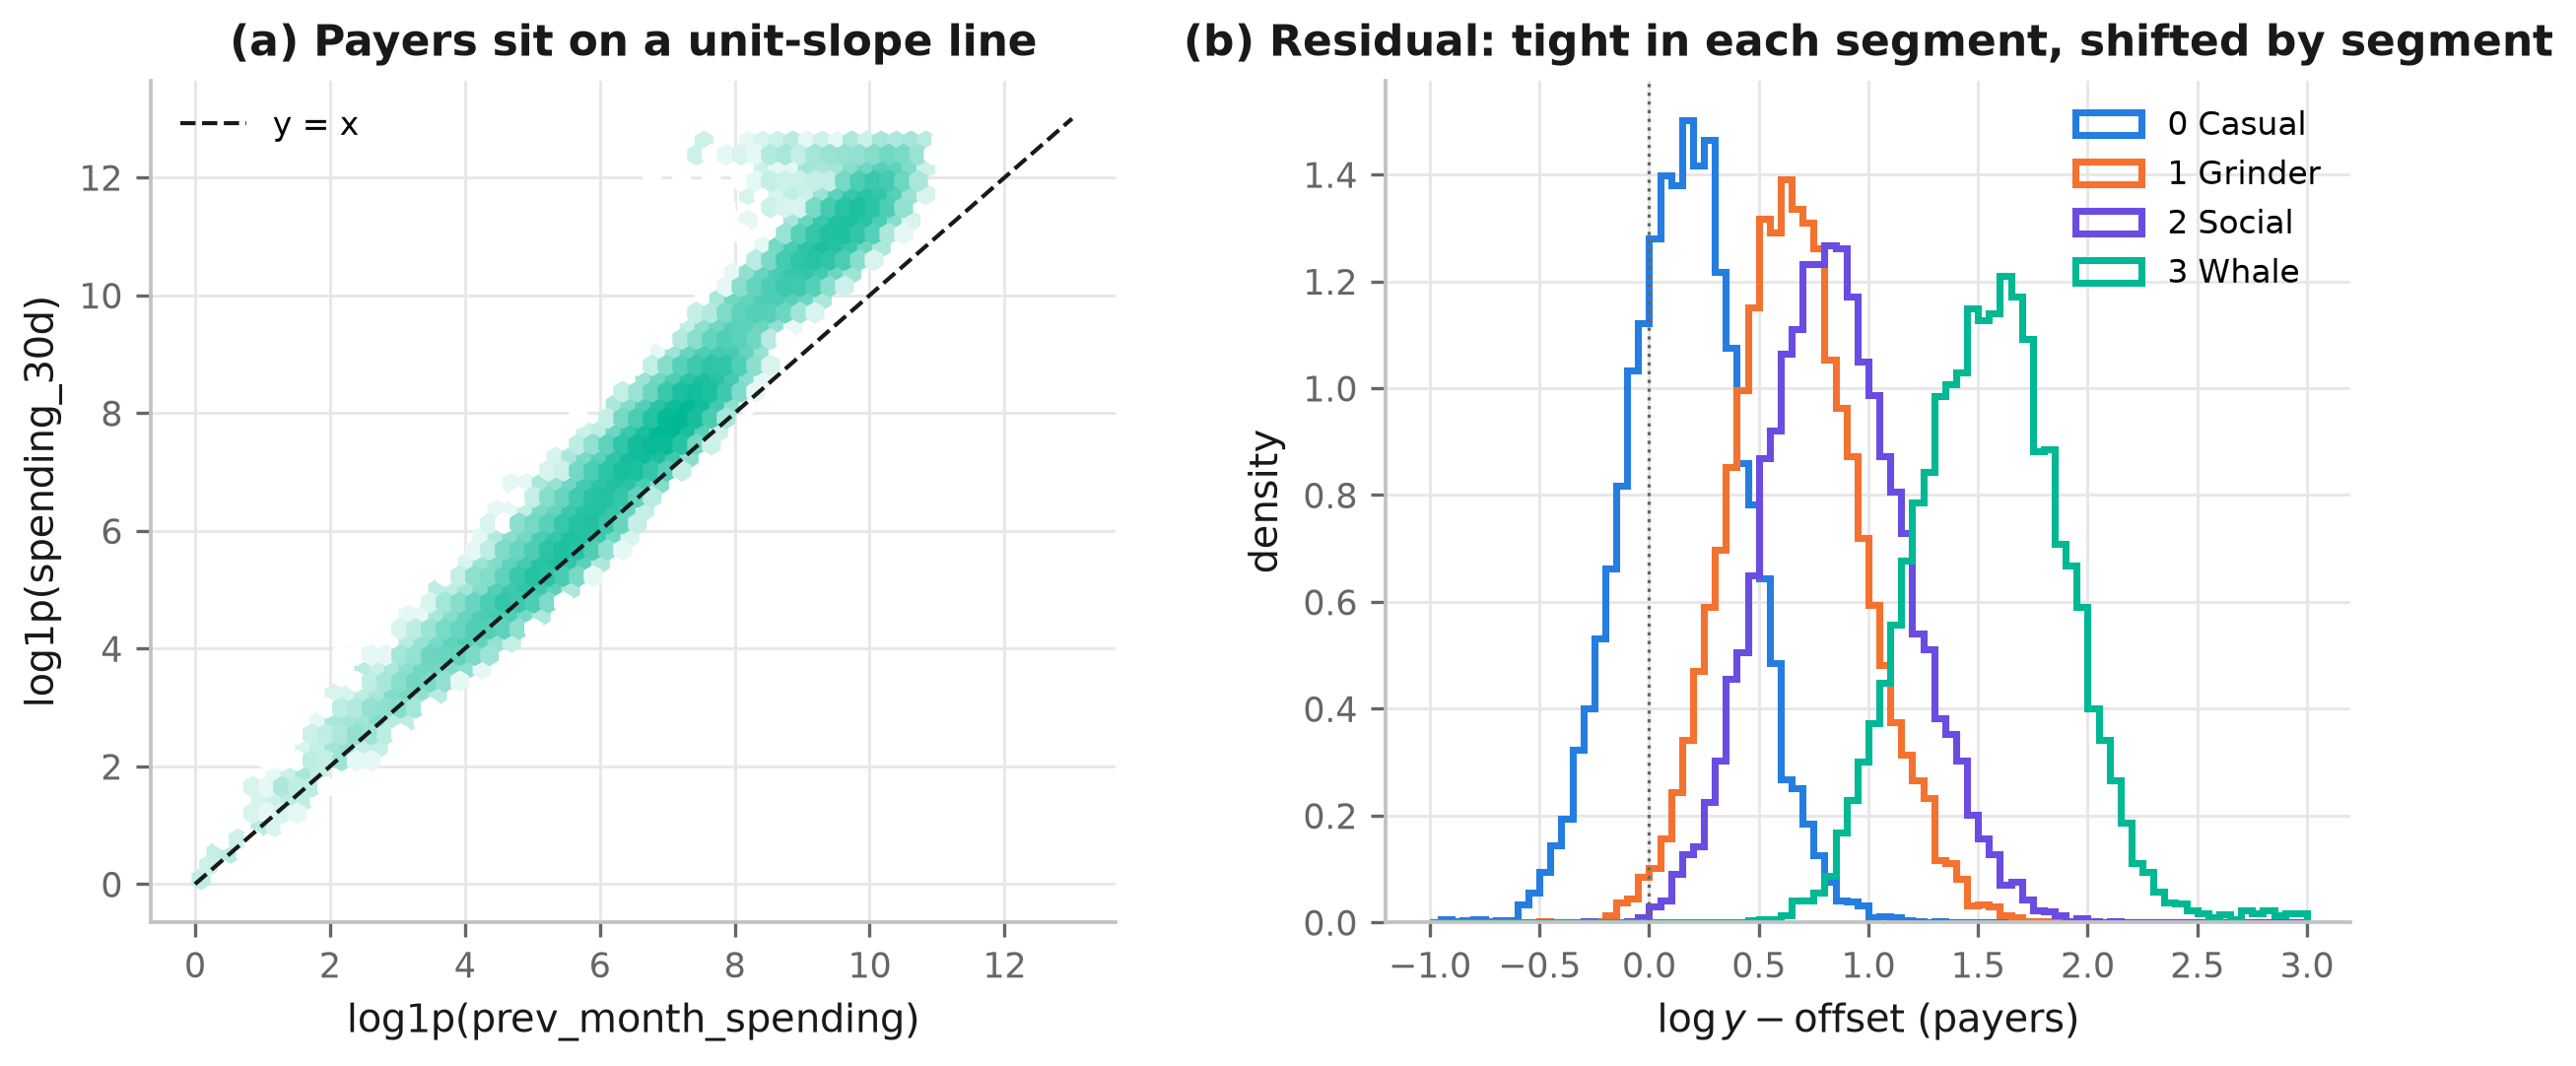
\includegraphics[width=\linewidth,height=0.33\textheight,keepaspectratio]{fig_t3_offset.png}
\caption{(a) Payers' $\log(1+y)$ against $\log(1+\texttt{prev\_month\_spending})$; the dashed line is $y=x$ and the flat edge at the top is the 300{,}000 cap. (b) The log-residual $\log y-\text{offset}$ by segment, with offset equal to $\log(1+\texttt{prev\_month\_spending})$.}
\label{fig:t3-offset}
\end{figure}

\emph{What we see.} For the 94\% of payers with a previous-month value, $\log y$ and $\log(1+\text{prev})$ have a correlation of 0.982, and the points lie on a band of slope one that is parallel to $y=x$ but above it. The residual is tight inside each segment (robust standard deviation 0.27--0.34) but its centre moves with the segment, from +0.17 for Casual to +1.56 for whales, and it carries further steps from premium status, VIP tier and recency. So last month is a strong anchor but not the whole answer. \emph{What we decided.} Model the \emph{residual} of the log amount against that anchor. A shallow tree model then only has to learn the multiplicative factors, not the whole scale of spending. Where \feat{prev_month_spending} is missing, the offset falls back to $\log(1+\text{historical})-1.05$, and finally to the constant 6.5.

\subsubsection{Data Preprocessing}

Table~\ref{tab:t3-evidence} links each figure to its decision, and the paragraphs below describe the steps in order.

\begin{evidencetable}{EDA evidence and the pipeline decision it motivated (task 3).}{tab:t3-evidence}
Figure~\ref{fig:t3-target}. 48\% zeros, payers across four orders of magnitude & Hurdle model: a payer probability $p$ and a payer-amount model on the log scale; point prediction chosen for MAE (Figure~\ref{fig:t3-qrule}). \\
Figure~\ref{fig:t3-whales}. Whales are 14\% of rows and 87\% of money & Impute the missing segment with an XGBoost classifier and add $P(\text{whale})$; judge changes by their effect on whales. \\
Figure~\ref{fig:t3-identities}. Exact products among five money columns & Iterative exact fill of the missing values, 5.8\% down to under 0.5\%. \\
Figure~\ref{fig:t3-offset}. Payers follow last month on a unit-slope line & Predict 11 quantiles of $\log y-\text{offset}$ with a depth-4 CatBoost model; offset from \feat{prev_month_spending}. \\
\end{evidencetable}

\paragraph{Exact fill.} Six rules fill a missing value from the other two in each identity: for example \feat{historical_spending} $=$ transactions $\times$ average value, transactions $=$ historical $/$ average value (only when the divisor is positive), and the analogous rules for the discount columns. Three passes let recovered values feed the next rule. The same function runs on train and test separately.

\paragraph{Derived features.} We add rates per day of account age (\feat{hist_per_day}, \feat{tx_per_day}), the expected monthly spend (\feat{avg_transaction_value} $\times$ \feat{purchase_frequency}), the ratios \feat{prev_vs_hist} and \feat{recency_ratio}, playtime per session, $\log(1+\cdot)$ of three money columns, and the number of missing values per row. The payer-amount model gets four more log-ratio features (previous minus historical, and so on).

\paragraph{Segment imputer.} An XGBoost~\citep{xgboost} multiclass model (depth 6, learning rate 0.02, early stopping on a 10\% holdout of the rows with a segment) predicts the missing segments from all other features. Its holdout accuracy is 0.9292. For each row we keep the imputed segment, a flag marking imputation, and the predicted probability of segment 3. The imputer sees only training rows and no target.

\paragraph{Folds.} Five stratified folds with seed 42, stratified jointly on ``zero'' and the four quartiles of the positive amounts, so that every fold holds the same mix of non-payers and small, medium and large payers.

\subsubsection{Model Design}
\label{sec:t3-design}

\paragraph{Why the median of the whole distribution.} MAE is minimised by the median of the predictive distribution, not by the mean. For a player with payer probability $p$, the whole distribution is a mass $1-p$ at zero plus $p$ times the payer distribution $F$. Its median $m$ solves $(1-p)+p\,F(m)=\tfrac12$. If $p\le\tfrac12$ the mass at zero already reaches one half and the median is $0$. If $p>\tfrac12$ the median is the payer quantile
\[
q=1-\frac{1}{2p}\in(0,\tfrac12],
\]
which is the lower half of the payer distribution, far below its mean. Figure~\ref{fig:t3-qrule}a draws the rule; Figure~\ref{fig:t3-qrule}b checks that $p$ can be trusted.

\begin{figure}[H]
\centering
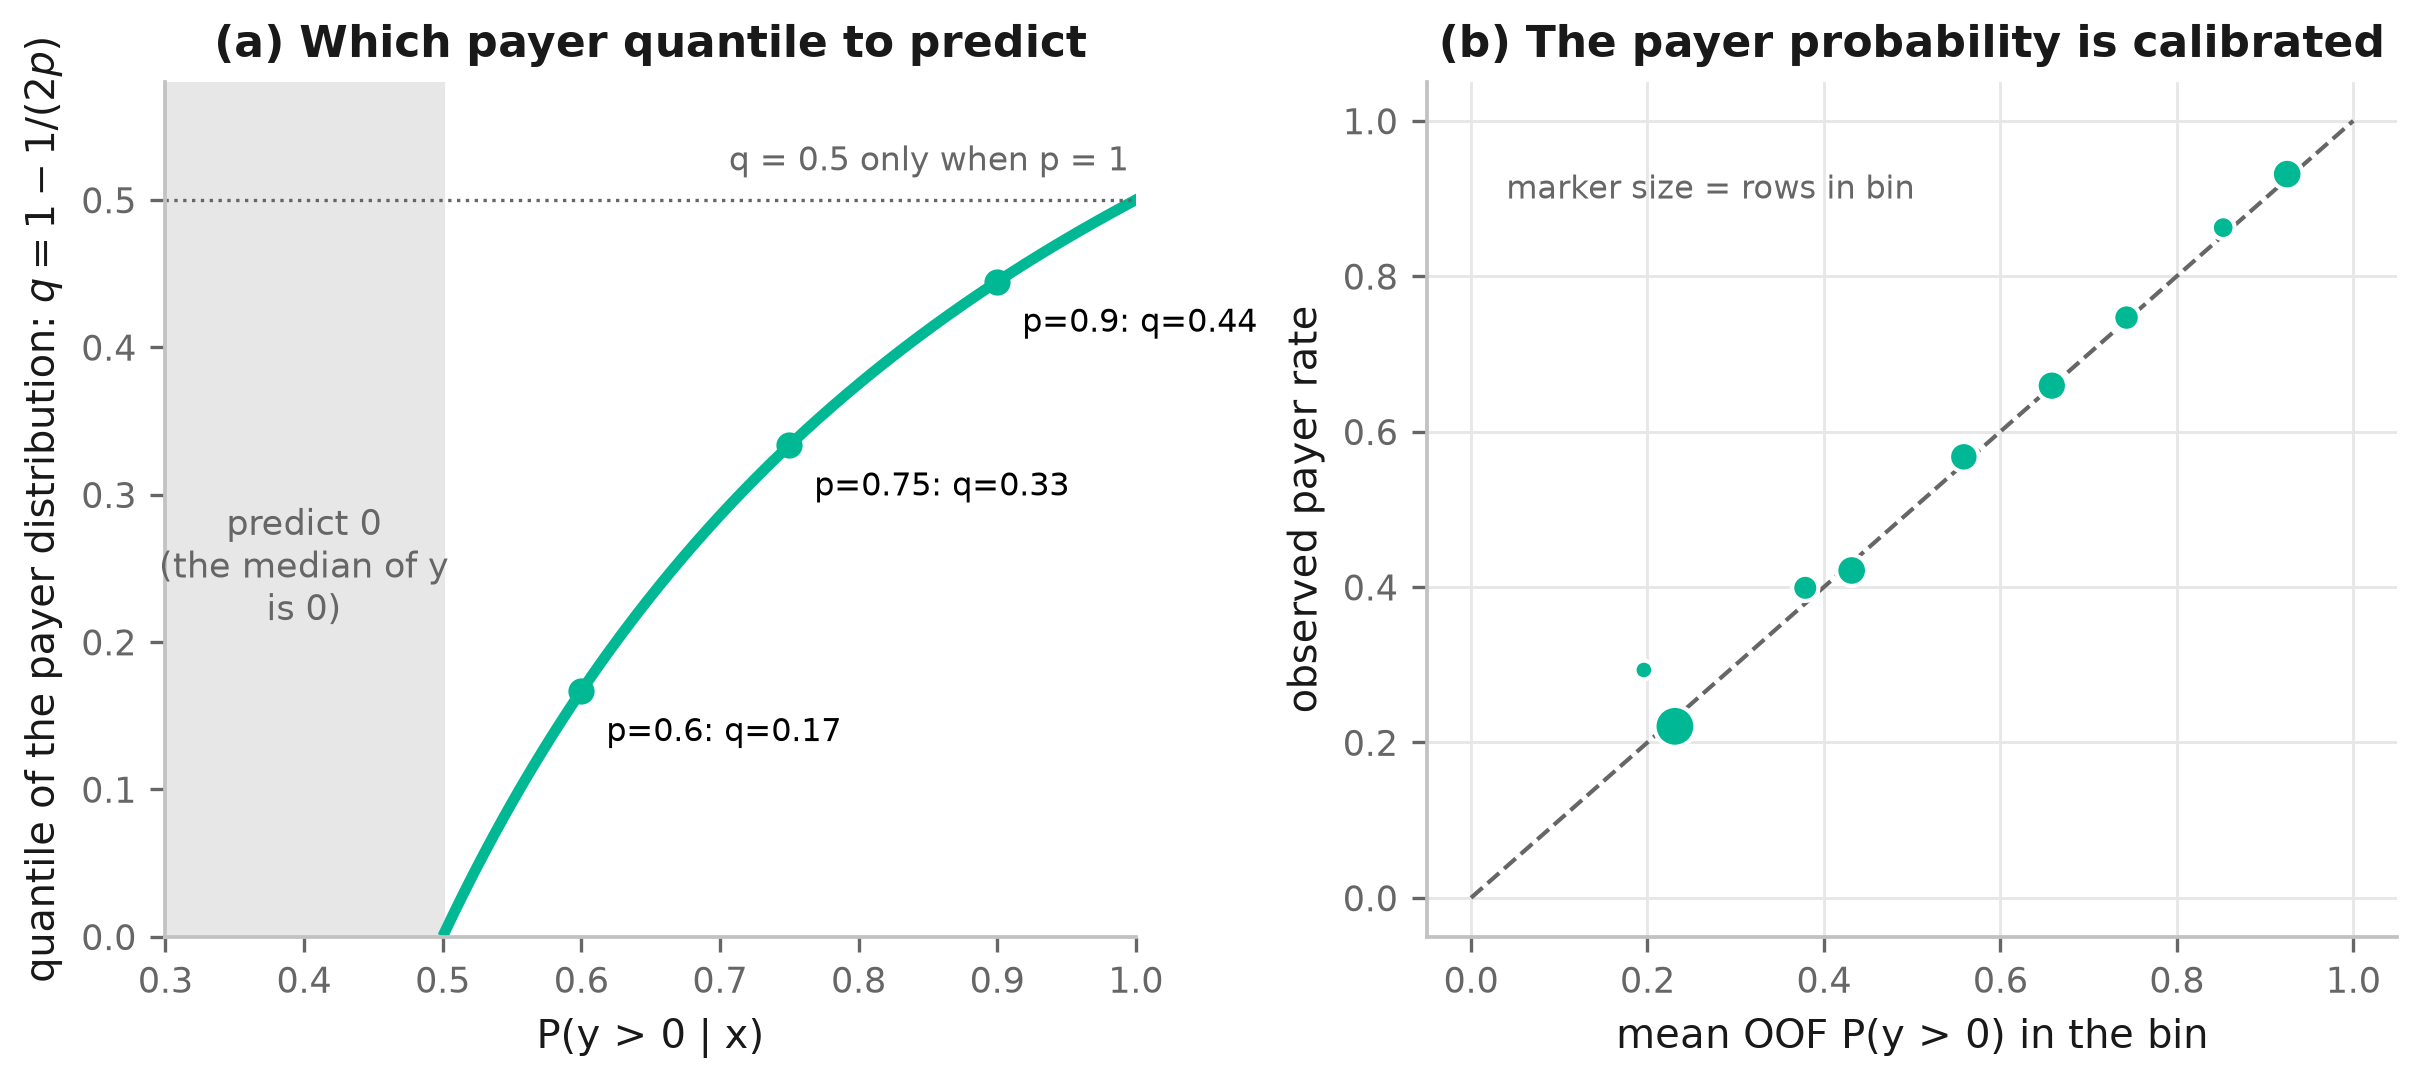
\includegraphics[width=\linewidth,height=0.33\textheight,keepaspectratio]{fig_t3_qrule.png}
\caption{(a) The payer quantile that minimises MAE as a function of $p=P(y>0\mid x)$; for $p\le0.5$ the best prediction is zero. (b) Reliability of the out-of-fold $p$ (10 bins; marker size is the number of rows): predicted and observed payer rates agree.}
\label{fig:t3-qrule}
\end{figure}

What this picture decides: the model must deliver (i) a calibrated $p$ and (ii) several quantiles of the payer amount below the median, because $q$ ranges from 0 to 0.5. A model of the mean would forecast the wrong quantity, a point we confirm in Section~\ref{sec:t3-eval}.

\paragraph{Architecture.} Figure~\ref{fig:t3-pipeline} shows the pipeline and Table~\ref{tab:t3-models} the settings. It is a hurdle model \citep{hurdle}: stage 1 is a LightGBM \citep{lightgbm} classifier, stage 2 a CatBoost \citep{catboost} model trained with the pinball (quantile) loss \citep{quantilereg}.

\begin{figure}[H]
\centering
\begin{tikzpicture}[x=1cm,y=1cm]
\node[stage] (raw) at (0,0) {Raw data\\104{,}000 rows, 32 features};
\node[stage,fill=\taskcolor{3}!14] (fill) at (5.4,0) {Exact identity fill (6 rules, 3 passes) and derived features};
\node[stage,fill=\taskcolor{3}!14] (seg) at (10.8,0) {Segment imputer (XGBoost, 92.9\% holdout) and $P(\text{whale})$};
\node[model,draw=\taskcolor{3},thick] (s1) at (0,-3.3) {\textbf{Stage 1: payer probability}\\LightGBM classifier, $p=P(y>0\mid x)$, 10 seeds $\times$ 5 folds};
\node[model,draw=\taskcolor{3},thick] (s2) at (5.4,-3.3) {\textbf{Stage 2: payer amount}\\CatBoost depth 4, 11 quantiles $0.02\ldots0.50$ of $\log y-\text{offset}$, payers only, 10 seeds $\times$ 5 folds};
\node[stage] (off) at (10.8,-3.3) {Offset: $\log(1+\text{prev})$, else $\log(1+\text{hist})-1.05$, else 6.5};
\node[decision,draw=\taskcolor{3},thick,text width=12cm] (dec) at (5.4,-5.9) {Hurdle median: $\hat y=0$ if $p\le 0.5$, else the payer quantile $q=1-1/(2p)$ read from the 11 quantiles by linear interpolation};
\node[stage,fill=\taskcolor{3}!14] (out) at (5.4,-7.8) {Predicted 30-day spending, clipped to $[0,300000]$};
\draw[flow] (raw) -- (fill);
\draw[flow] (fill) -- (seg);
\coordinate (bus) at (10.8,-1.6);
\draw[thick,ink!75] (seg.south) -- (bus);
\draw[thick,ink!75] (bus) -- (0,-1.6);
\draw[flow] (0,-1.6) -- (s1.north);
\draw[flow] (5.4,-1.6) -- (s2.north);
\draw[flow] (off) -- (s2);
\draw[flow] (s1.south) -- (s1.south |- dec.north);
\draw[flow] (s2.south) -- (s2.south |- dec.north);
\draw[flow] (dec) -- (out);
\node[note,anchor=north] at (5.4,-8.5) {$p$ is averaged over seeds; the quantiles are averaged by geometric mean on the baht scale};
\end{tikzpicture}
\caption{Task 3 pipeline from raw features to predicted spending.}
\label{fig:t3-pipeline}
\end{figure}

\begin{table}[H]\centering\small
\caption{Components of the final Task 3 model.}\label{tab:t3-models}
\begin{tabular}{@{}L{.20\linewidth}L{.74\linewidth}@{}}
\toprule
\textbf{Component} & \textbf{Settings} \\
\midrule
Stage 1, payer probability & LightGBM binary classifier: learning rate 0.03, 63 leaves, minimum 40 rows per leaf, row and column subsampling 0.8 and 0.7, $\ell_2=2$; early stopping (100 rounds) on 10\% of each training fold. 45 features. Ten seeds $\times$ five folds; the 10 seed predictions are averaged. \\
Stage 2, payer amount & CatBoost \texttt{MultiQuantile} on the payers of each fold, target $\log y-\text{offset}(x)$, quantile levels 0.02, 0.05, 0.10, \ldots, 0.50 (11 levels); depth 4, learning rate 0.05, $\ell_2=3$, up to 20{,}000 iterations with overfitting detector (200). 49 features. Ten seeds $\times$ five folds; the predicted quantiles are sorted and averaged by geometric mean over seeds. \\
Point prediction & $q=\mathrm{clip}\bigl(1-1/(2p),0.02,0.50\bigr)$, linear interpolation between neighbouring quantile levels, $\hat y=0$ where $p\le0.5$, clipped to $[0,300000]$. \\
\bottomrule
\end{tabular}
\end{table}

\paragraph{Why these choices.} \emph{Depth 4.} The log-residual is a sum of a few multiplicative steps (premium, VIP tier, number of games, recency, month), which shallow symmetric trees represent well. Figure~\ref{fig:t3-sweep}a and the paragraph below give the sweep: CatBoost is flat from depth 3 to 6 and falls at depth 8, XGBoost \citep{xgboost} is lower at every depth, and LightGBM is lower again. \emph{Multi-quantile.} One model produces all 11 quantiles together with shared trees; the predicted quantiles are sorted afterwards to remove any crossing. \emph{Seeds.} The seed average costs compute only: ten seeds of each stage added 0.00006 over three of each.

\paragraph{Model family and depth sweep.} All amount-model variants share the exact fill, the offset target, the 49 features, the five folds and the same stage-1 probabilities, so only the booster changes (Figure~\ref{fig:t3-sweep}a; one seed per point, data in \texttt{data/t3\_sweep.csv}).

\begin{figure}[H]
\centering
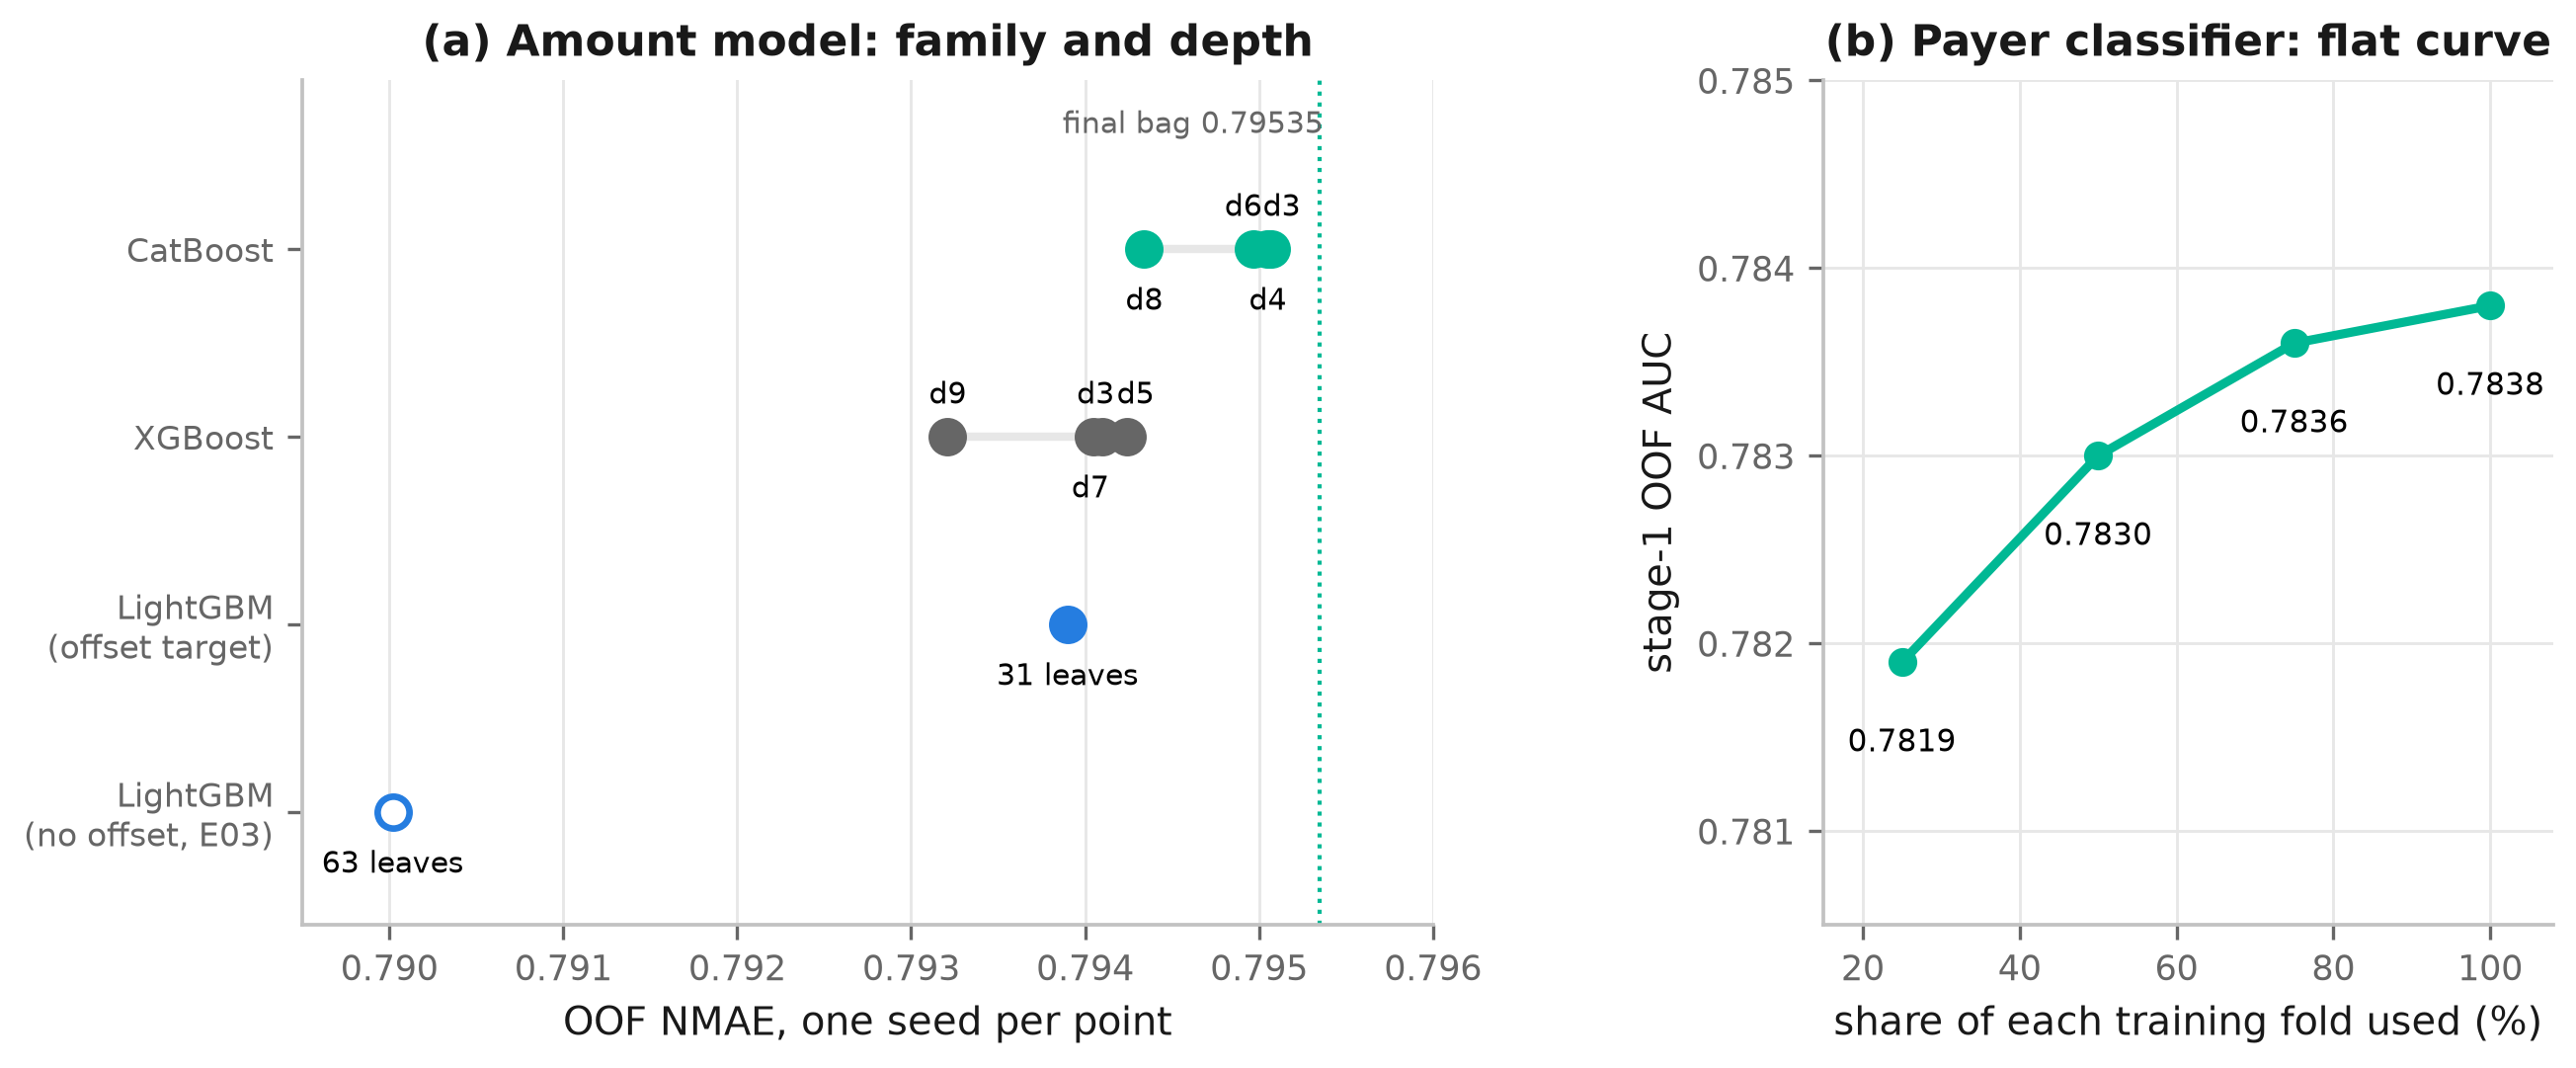
\includegraphics[width=\linewidth,height=0.33\textheight,keepaspectratio]{fig_t3_sweep.png}
\caption{(a) OOF NMAE of the amount model by family and depth (CatBoost, XGBoost and LightGBM with the offset target, plus LightGBM without it; experiments E03, E07, E12, E15, E16, E26, E29, E30, E32, E34 of the research log). (b) Stage-1 AUC as the training folds are subsampled: the curve is nearly flat.}
\label{fig:t3-sweep}
\end{figure}

\emph{What we see.} CatBoost scores 0.79507, 0.79505, 0.79497 and 0.79434 at depths 3, 4, 6 and 8: flat up to depth 6 and 0.0007 lower at depth 8. XGBoost, with the same offset and features, scores 0.79410, 0.79424, 0.79405 and 0.79321 at depths 3, 5, 7 and 9, so its best depth is 5 and it stays 0.0008 or more below CatBoost. (The XGBoost depth-7 point is the offset run E07; the same depth without the offset target scored 0.79162, E05.) A LightGBM hurdle with one regression per quantile level scores 0.79002 without the offset target (E03), which is 0.0016 below XGBoost without it, and 0.79390 with the offset (E26). Learning rate differs slightly between the CatBoost runs (0.04 to 0.06), and every difference between depths 3 and 6 is far below the fold standard deviation of 0.0076. \emph{What we decided.} Depth 4 CatBoost: it is the cheapest of the flat region and the best single model. In a bag, XGBoost added no diversity once CatBoost was shallow (three CatBoost depth-4 models plus three XGBoost depth-5 models scored 0.79517, against 0.79529 for CatBoost alone; E38, E35).

\emph{Choice of the stage-1 classifier.} Training the classifier on 25, 50, 75 and 100\% of each training fold gives an out-of-fold AUC of 0.7819, 0.7830, 0.7836 and 0.7838 (Figure~\ref{fig:t3-sweep}b), so more data would add little. CatBoost depth 6, CatBoost depth 4 and XGBoost classifiers reach AUC 0.78446, 0.78443 and 0.78413 against 0.78409 for the three-seed LightGBM, and swapping or mixing them into the final model moves the NMAE by +0.00002 (0.79531 against 0.79529), which is noise. We kept LightGBM, which is the fastest.

\paragraph{Earlier model: the ZILN hurdle.} Before the CatBoost quantile model, our Task~3 submissions \texttt{sub\_v5} and \texttt{sub\_v6} used a blend built on a \emph{zero-inflated log-normal} (ZILN) model (Section~\ref{sec:t3-eval}). ZILN writes the target as a mass at zero plus a log-normal payer amount and fits both parts with one likelihood. With $z_i=\log(1+y_i)$, $p_i=P(y_i>0\mid x_i)$ and a mixture of $K$ log-normals for the payer amount, the loss we minimised on the training rows is
\[
\mathcal L=\underbrace{-\tfrac1n\sum_i\bigl[\mathbf{1}(y_i{=}0)\log(1-p_i)+\mathbf{1}(y_i{>}0)\log p_i\bigr]}_{\text{binary cross-entropy on paying}}
\;\underbrace{-\;\tfrac1n\sum_{i:\,y_i>0}\log\sum_{k=1}^{K}\pi_{ik}\,\mathcal N\!\bigl(z_i;\mu_{ik},\sigma_{ik}^2\bigr)}_{\text{log-normal NLL of the payers}} ,
\]
which is the loss of Wang et al.\ (2019)~\citep{ziln} for $K=1$. It fits this target for the two reasons of Section~\ref{sec:t3-eda}: 48\% of the rows are exact zeros, and the payer amount is a product of several factors, so $\log y$ is the natural scale. We ran it in two forms, both on the same exact fill, segment imputer and folds as the final model. In the \emph{gradient-boosting form} (notebooks \texttt{task3-hurdle-ziln}, versions 1 to 3, and \texttt{task3-hurdle-ziln-v4}) XGBoost fitted $p$ with a classifier, the mean $\mu(x)$ of $\log(1+y)$ for payers with a squared-error regressor, and the log-variance with a second regressor, with a log-normal as the payer law. In the \emph{neural form} (\texttt{task3-nn-ziln}) one network predicts $p$, the weights $\pi_k$, the means $\mu_k$ and the scales $\sigma_k$ jointly. It embeds each quantile-normalised numeric feature with periodic features, passes them through three residual blocks of width 512, and was trained with AdamW, one-cycle learning rate, at most 80 epochs and early stopping on 10\% of each fold, two seeds per fold. $K=1$ is plain ZILN and $K=3$ is a mixture of three log-normals.

The point prediction is the hurdle median derived at the start of this section. Both forms return a full payer distribution, so we set $\hat y=0$ when $p\le\tfrac12$ and otherwise take its quantile at $q=1-1/(2p)$: for the single log-normal that is $\exp(\mu+\sigma\,\Phi^{-1}(q))-1$, for the mixture we invert the mixture cdf by bisection. Two numbers, a shift of $p$ and a multiplicative scale, were tuned on the out-of-fold predictions (for the $K=3$ network the shift is $+0.05$ and the scale $0.975$). The ZILN stack was then blended with the XGBoost multi-quantile models (Section~\ref{sec:t3-eval}). The ZILN branch was later replaced by direct quantile models, and the analysis of the data generator explains why a parametric shape for every player is a poor fit (Sections~\ref{sec:t3-eval} and~\ref{sec:t3-mistakes}). The ZILN runs used the first data release; Task~3 was not changed by the re-release of 12 November, so these scores are comparable with the final ones.

\subsubsection{Evaluation and Results}
\label{sec:t3-eval}

Table~\ref{tab:t3-results} follows the out-of-fold score from the first hurdle model to the final one, and Figure~\ref{fig:t3-progress} draws the same steps. All numbers use the same five folds. The final row is the value printed by the submission notebook.

\begin{table}[H]\centering\small
\caption{Out-of-fold NMAE score at each milestone (5 folds, seed 42). Rows above the last come from the local research pipeline with the same folds; the last row is the submission notebook.}\label{tab:t3-results}
\begin{tabular}{@{}L{.56\linewidth}L{.15\linewidth}L{.20\linewidth}@{}}
\toprule
\textbf{Model} & \textbf{OOF NMAE} & \textbf{Change vs row above} \\
\midrule
Two-stage hurdle, gradient boosting (HGB) & 0.7843 & --- \\
XGBoost multi-quantile hurdle, nested LAD blend & 0.79191 & +0.00761 \\
XGBoost on $\log(y/\text{prev})$ offset & 0.79391 & +0.00200 \\
XGBoost offset + 4 log-ratio features & 0.79405 & +0.00014 \\
CatBoost depth 4, offset, one seed & 0.79505 & +0.00100 \\
CatBoost + LightGBM, $3\times3$ seeds & 0.79529 & +0.00024 \\
\textbf{Final, $10\times10$ seeds (notebook)} & \textbf{0.79535} & +0.00006 \\
\bottomrule
\end{tabular}
\end{table}

\begin{figure}[H]
\centering
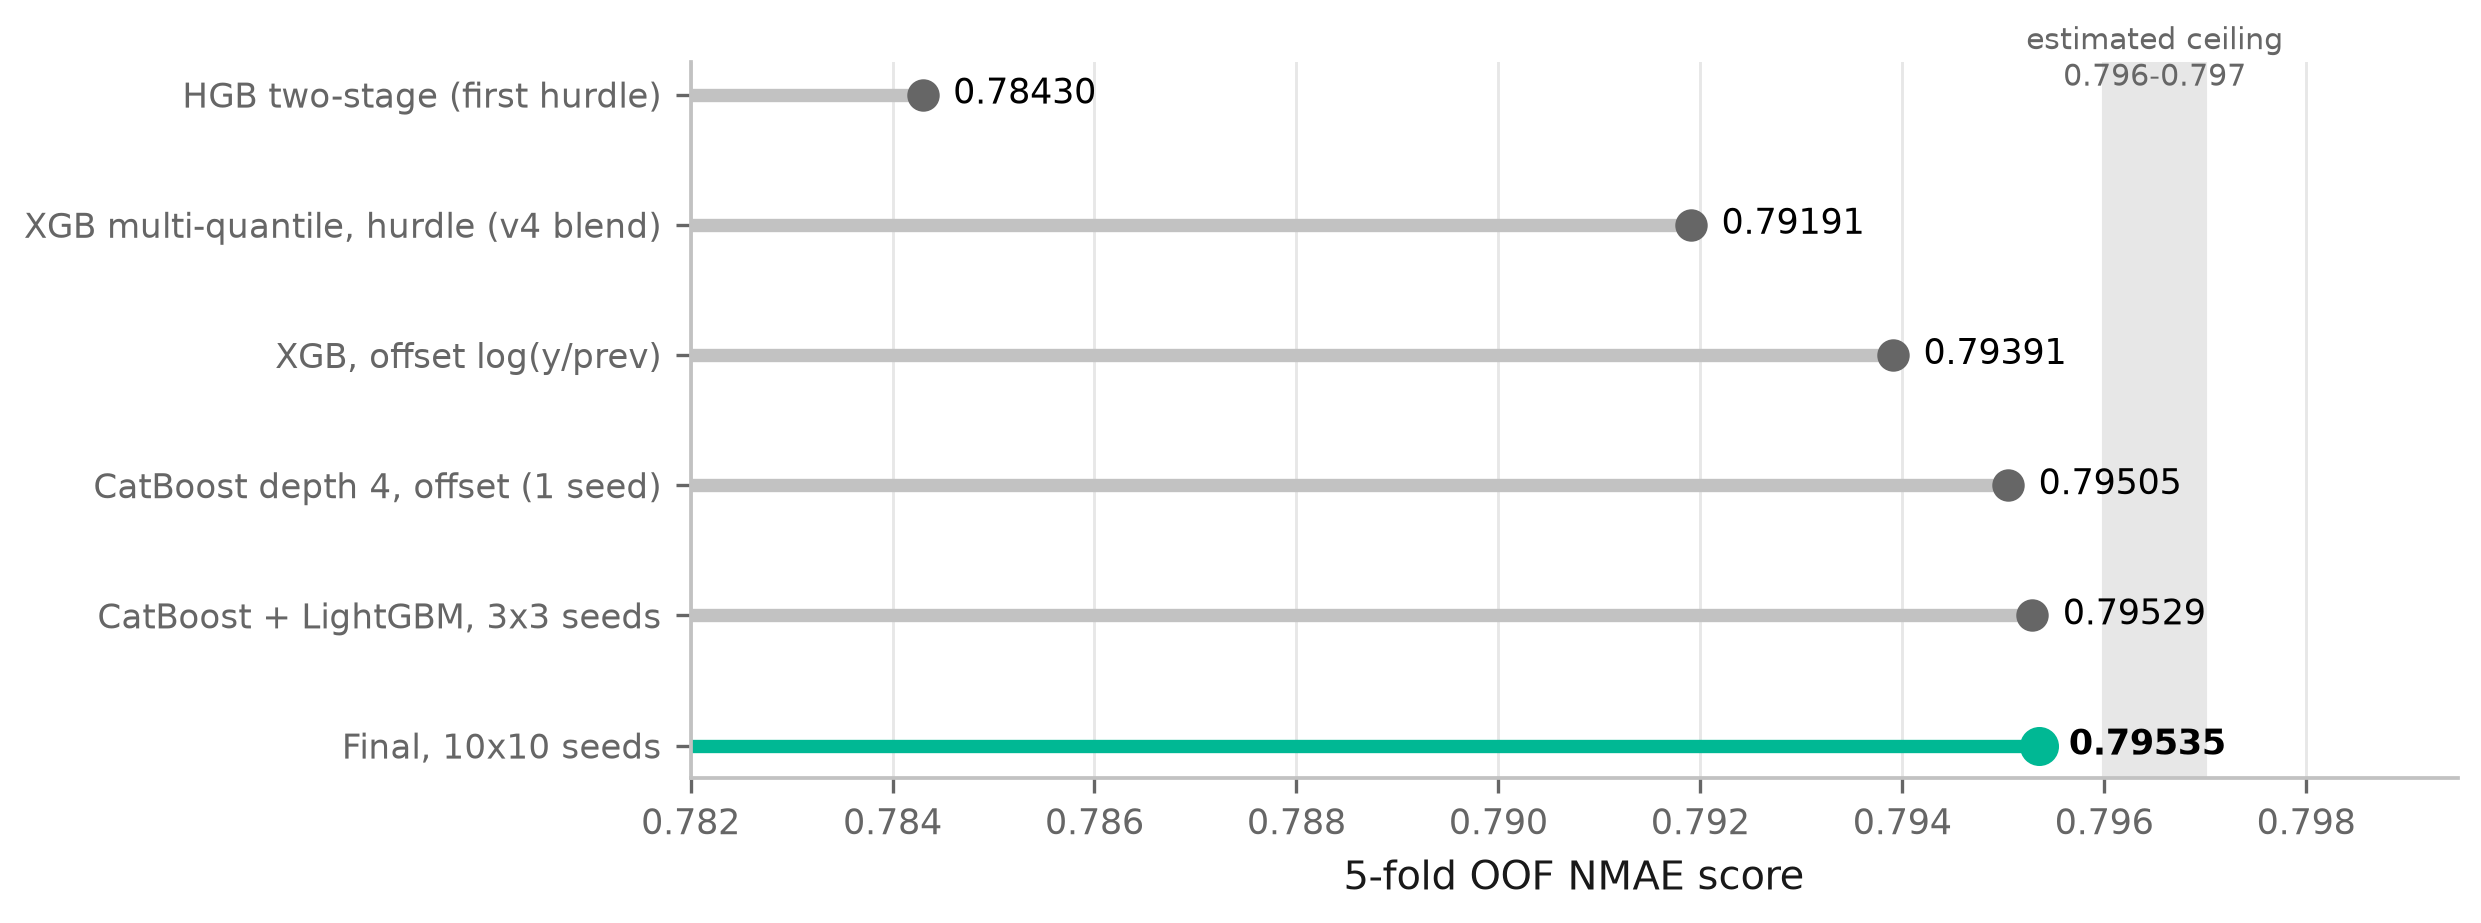
\includegraphics[width=.85\linewidth]{fig_t3_progression.png}
\caption{OOF NMAE of each milestone. The shaded band is the ceiling that the learning curve of the payer residual suggests (0.796--0.797); the last three steps add less than 0.0013 together.}
\label{fig:t3-progress}
\end{figure}

The final model scores 0.79535 (fold mean 0.79540, standard deviation 0.0076 across folds; the saved 10$\times$10 ensemble from the research pipeline gives 0.79537). Stage 1 alone reaches an out-of-fold AUC of 0.78439. The model predicts zero for 50.4\% of test players and has a mean prediction of 10{,}430 THB, close to the training mean of 10{,}497 THB. In the public leaderboard the 10-seed version scored 0.00001 above the 3-seed one (\texttt{sub\_v24a} against \texttt{sub\_v23a}), as the out-of-fold gain predicted.

\paragraph{How the model evolved, including the ZILN stages.} Figure~\ref{fig:t3-evolution} places the earlier ZILN stages on the same scale (data in \texttt{data/t3\_model\_evolution.csv}). The first hurdle ZILN model (XGBoost with a log-normal payer head) scored 0.7893, version 2 with the exact fill and the segment imputer 0.7916, version 3 0.7917, and the version-4 XGBoost multi-quantile blend 0.7920 (weights tuned on the same out-of-fold rows; the nested value is 0.79191 in Table~\ref{tab:t3-results}). The neural ZILN reached 0.7867 with one log-normal and 0.7901 with three. Blending version 4 with the $K=3$ network (weights 0.38, 0.24, 0.06 for the three XGBoost quantile models and 0.32 for the network) gave 0.7925 with in-sample weights; that blend was the Task~3 column of \texttt{sub\_v5} and \texttt{sub\_v6}. The CatBoost offset model then reached 0.79505 alone and 0.79535 as the final bag.

\begin{figure}[H]
\centering
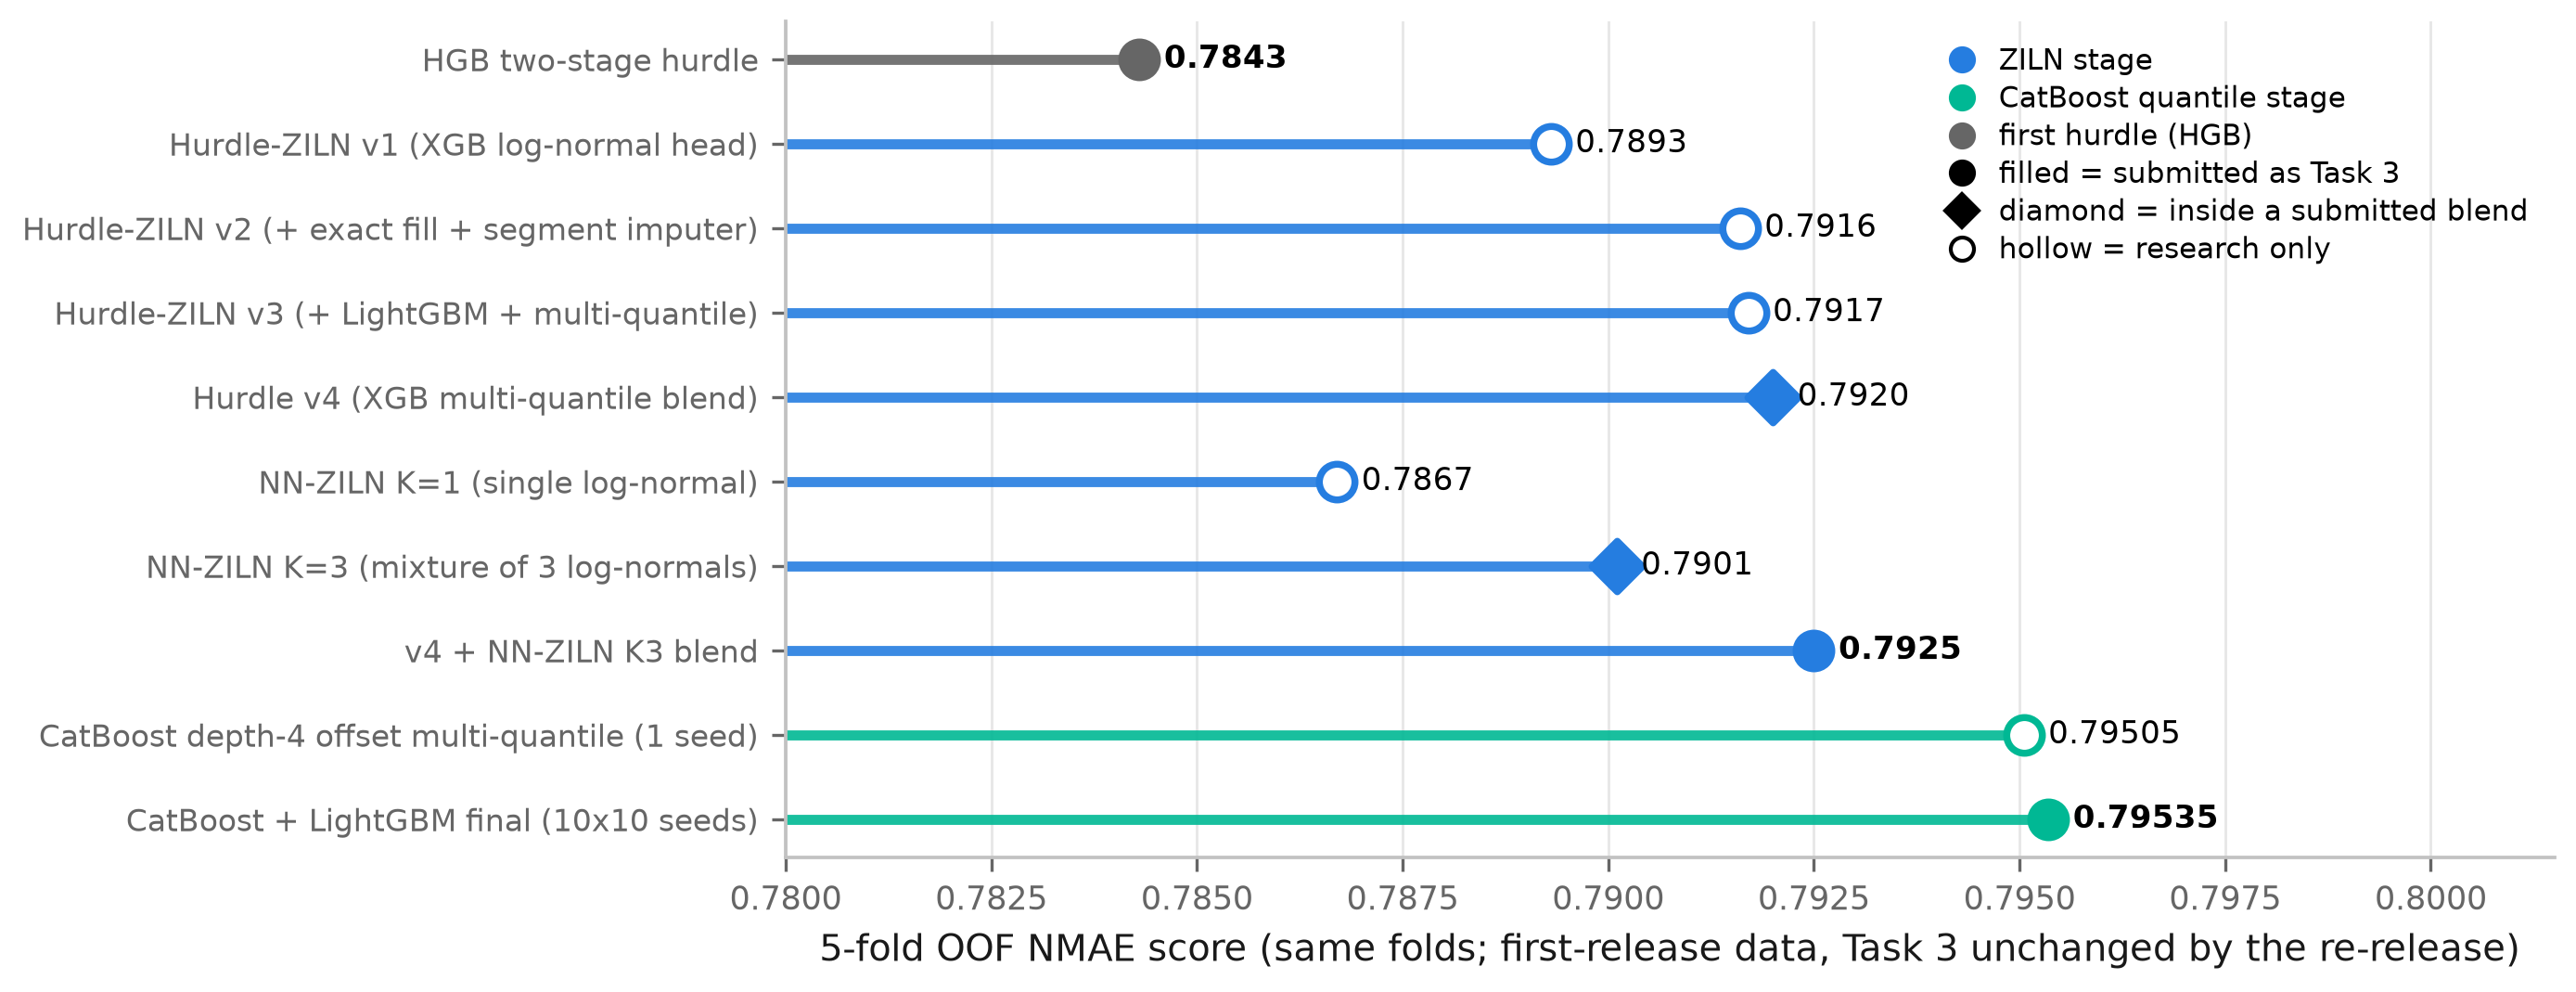
\includegraphics[width=\linewidth,height=0.38\textheight,keepaspectratio]{fig_t3_evolution.png}
\caption{OOF NMAE of every Task~3 modelling stage. Blue marks the ZILN stages, green the CatBoost quantile stages. Filled markers were submitted as Task~3, diamonds were components of a submitted blend, hollow markers were research runs only. The ZILN stack reached 0.7925; the quantile model that replaced it is 0.0029 higher.}
\label{fig:t3-evolution}
\end{figure}

What we see: each ZILN stage gained from better inputs (exact fill, segment) and from a better payer law (mixture instead of one log-normal), until about 0.792; the move from a parametric payer law to direct quantiles, an offset target and CatBoost added about 0.003, ten times the later seed averaging. What we decided: stop developing the ZILN branch and keep the hurdle rule, which both families share.

\paragraph{Baselines.} Table~\ref{tab:t3-baselines} gives simple predictors on the same training rows, to show what the score means. A constant mean scores below the all-zero baseline because MAE punishes the many small payers it overpredicts and the whales it underpredicts.

\begin{table}[H]\centering\small
\caption{NMAE score of simple predictors on the training rows (no model fitting except the medians).}\label{tab:t3-baselines}
\begin{tabular}{@{}L{.62\linewidth}L{.15\linewidth}@{}}
\toprule
\textbf{Predictor} & \textbf{NMAE} \\
\midrule
Predict the overall mean for everyone & 0.3861 \\
Predict zero for everyone & 0.5000 \\
Previous month's spending & 0.5452 \\
Median spending of the player's segment & 0.6139 \\
\textbf{Final model (OOF)} & \textbf{0.7954} \\
\bottomrule
\end{tabular}
\end{table}

\paragraph{The decision rule matters.} Table~\ref{tab:t3-rule} replaces the rule on the saved out-of-fold probabilities and quantiles.

\begin{table}[H]\centering\small
\caption{Alternative point-prediction rules applied to the same OOF probabilities and quantiles (saved 10$\times$10 ensemble).}\label{tab:t3-rule}
\begin{tabular}{@{}L{.62\linewidth}L{.15\linewidth}L{.15\linewidth}@{}}
\toprule
\textbf{Rule} & \textbf{OOF NMAE} & \textbf{vs final} \\
\midrule
\textbf{$q=1-1/(2p)$, zero if $p\le0.5$ (final)} & \textbf{0.79537} & --- \\
Same rule, zero if $p\le0.45$ & 0.79528 & $-0.00009$ \\
Same rule, zero if $p\le0.55$ & 0.79503 & $-0.00034$ \\
Same rule, zero if $p\le0.40$ / $0.60$ & 0.79468 / 0.79413 & $-0.00069$ / $-0.00124$ \\
Median of the payer distribution ($q=0.5$), zero if $p\le0.5$ & 0.79427 & $-0.00110$ \\
Never predict zero, payer median & 0.78990 & $-0.00547$ \\
$p\times$ payer median (expected-value style) & 0.78682 & $-0.00855$ \\
\bottomrule
\end{tabular}
\end{table}

\paragraph{Post-hoc (shift, kappa) calibration.} A hurdle rule is only optimal if $p$ and the quantiles are calibrated, so the first thing we tried on top of every model was a two-parameter correction fitted on out-of-fold predictions: shift the probability, $p'=p+s$, and scale the predicted amount, $\hat y'=\kappa\hat y$. We repeated it in seven variants (global and per-segment shift and kappa, a shift of the quantile level instead of $p$, a scale per prediction decile, a scale per segment and prediction bin, and zeroing predictions below a cut-off $c$), each tuned on four folds and applied to the fifth. Figure~\ref{fig:t3-paired} (top panel) shows that all land within $\pm0.00001$ of the uncalibrated final model (0.79529, experiments R3-A to R3-G; paired standard deviation 0.00002--0.00005). The fitted parameters sit at the identity, about $(s,\kappa)=(0.02,1.00)$, the decile scales lie between 0.99 and 1.01, the cut-off picks $c=0$, and for the LightGBM hurdle each segment picks shift 0 and kappa 1 (E04). This is the numerical form of the reliability plot in Figure~\ref{fig:t3-qrule}b: the model is already calibrated, and the median rule leaves nothing for post-processing to correct. \emph{Decision.} No calibration step in the final model; this also removes a tuned parameter that would have needed nesting.

\paragraph{Fold-seed robustness.} To check that the gain of the final recipe over our earlier XGBoost model is not luck of one fold split, we redrew the five folds with seed 7 (R2-09). The comparison is between two recipes, not two seeds of one: the earlier XGBoost multi-quantile model without the offset target (0.79183) and the final recipe, CatBoost depth 4 with the offset (0.79531), one seed each and the same stage-1 probabilities. The paired gain is $+0.00348\pm0.00045$ and positive in 5 of 5 folds, against $+0.00344$ on the original folds. So the gain comes from the model and the offset, not from the fold split.

\paragraph{Decision log.} Figure~\ref{fig:t3-decision-log} lists every Task~3 experiment with its metric; the rows are in \texttt{data/decision\_log\_t3.csv}.

\begin{figure}[p]
\centering
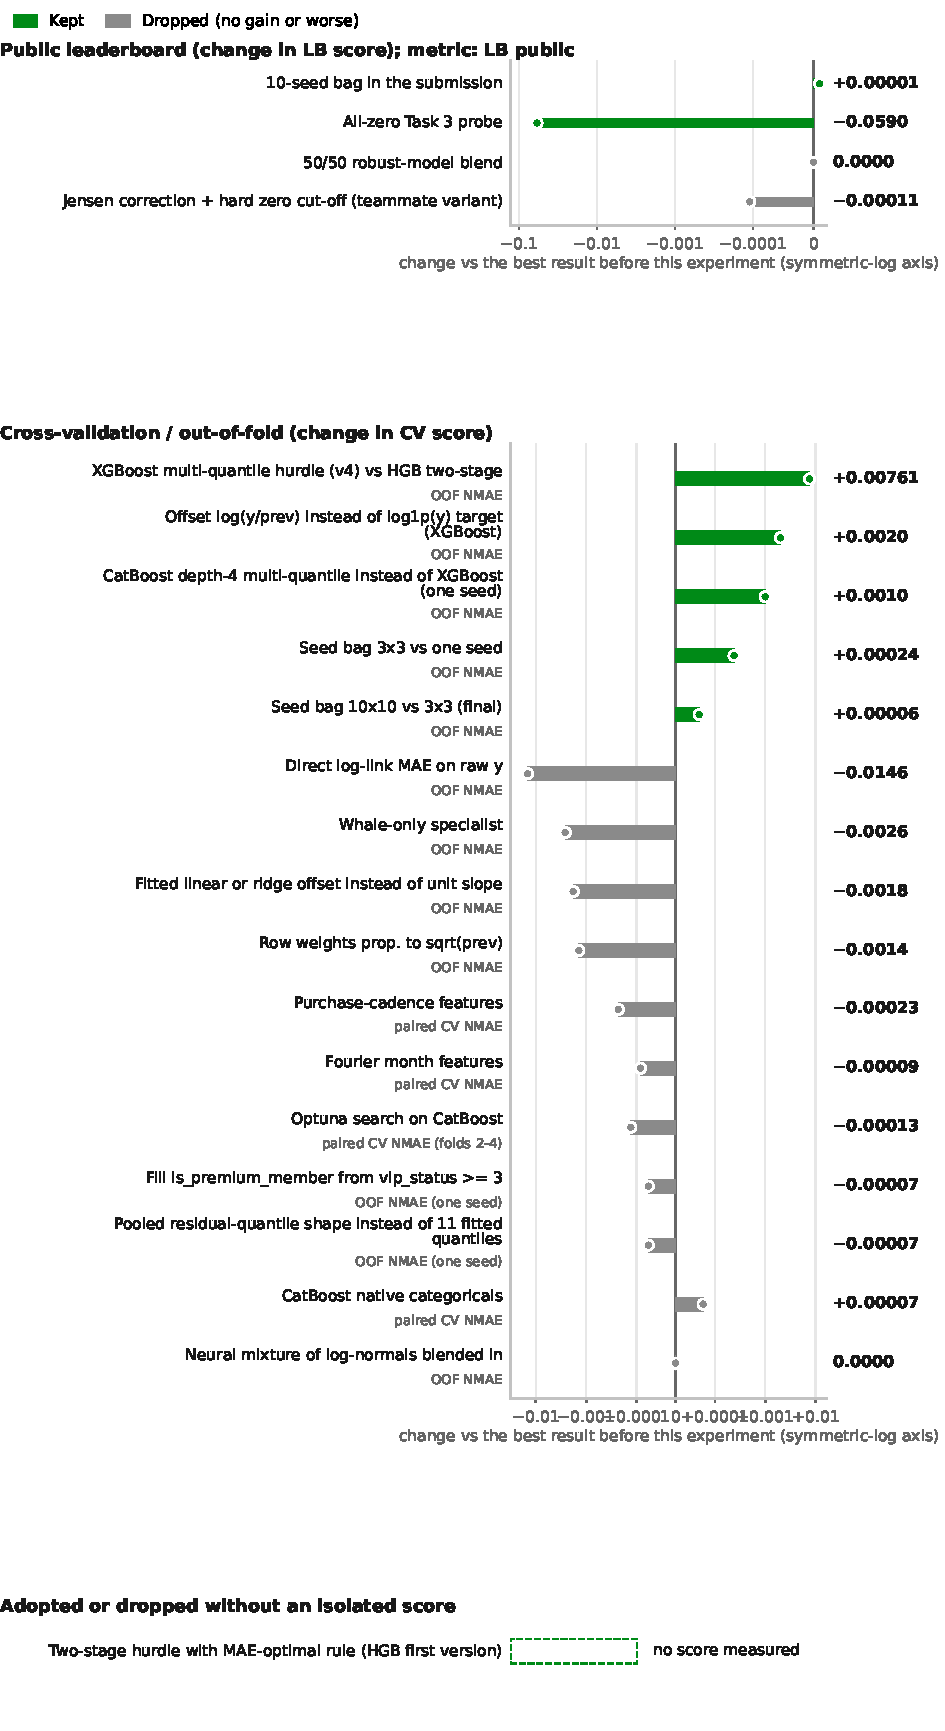
\includegraphics[width=\linewidth,height=0.85\textheight,keepaspectratio]{decision_log_t3.pdf}
\caption{Task 3 decision log: change in score (one panel per metric family) per experiment, kept versus dropped versus rule-excluded. Green = kept, grey = dropped, red hatched = excluded by the competition rules.}
\label{fig:t3-decision-log}
\end{figure}

\subsubsection{Insights from Model Behaviour}

\paragraph{Where the error sits.} Figure~\ref{fig:t3-error} splits the out-of-fold absolute error by segment and by source.

\begin{figure}[H]
\centering
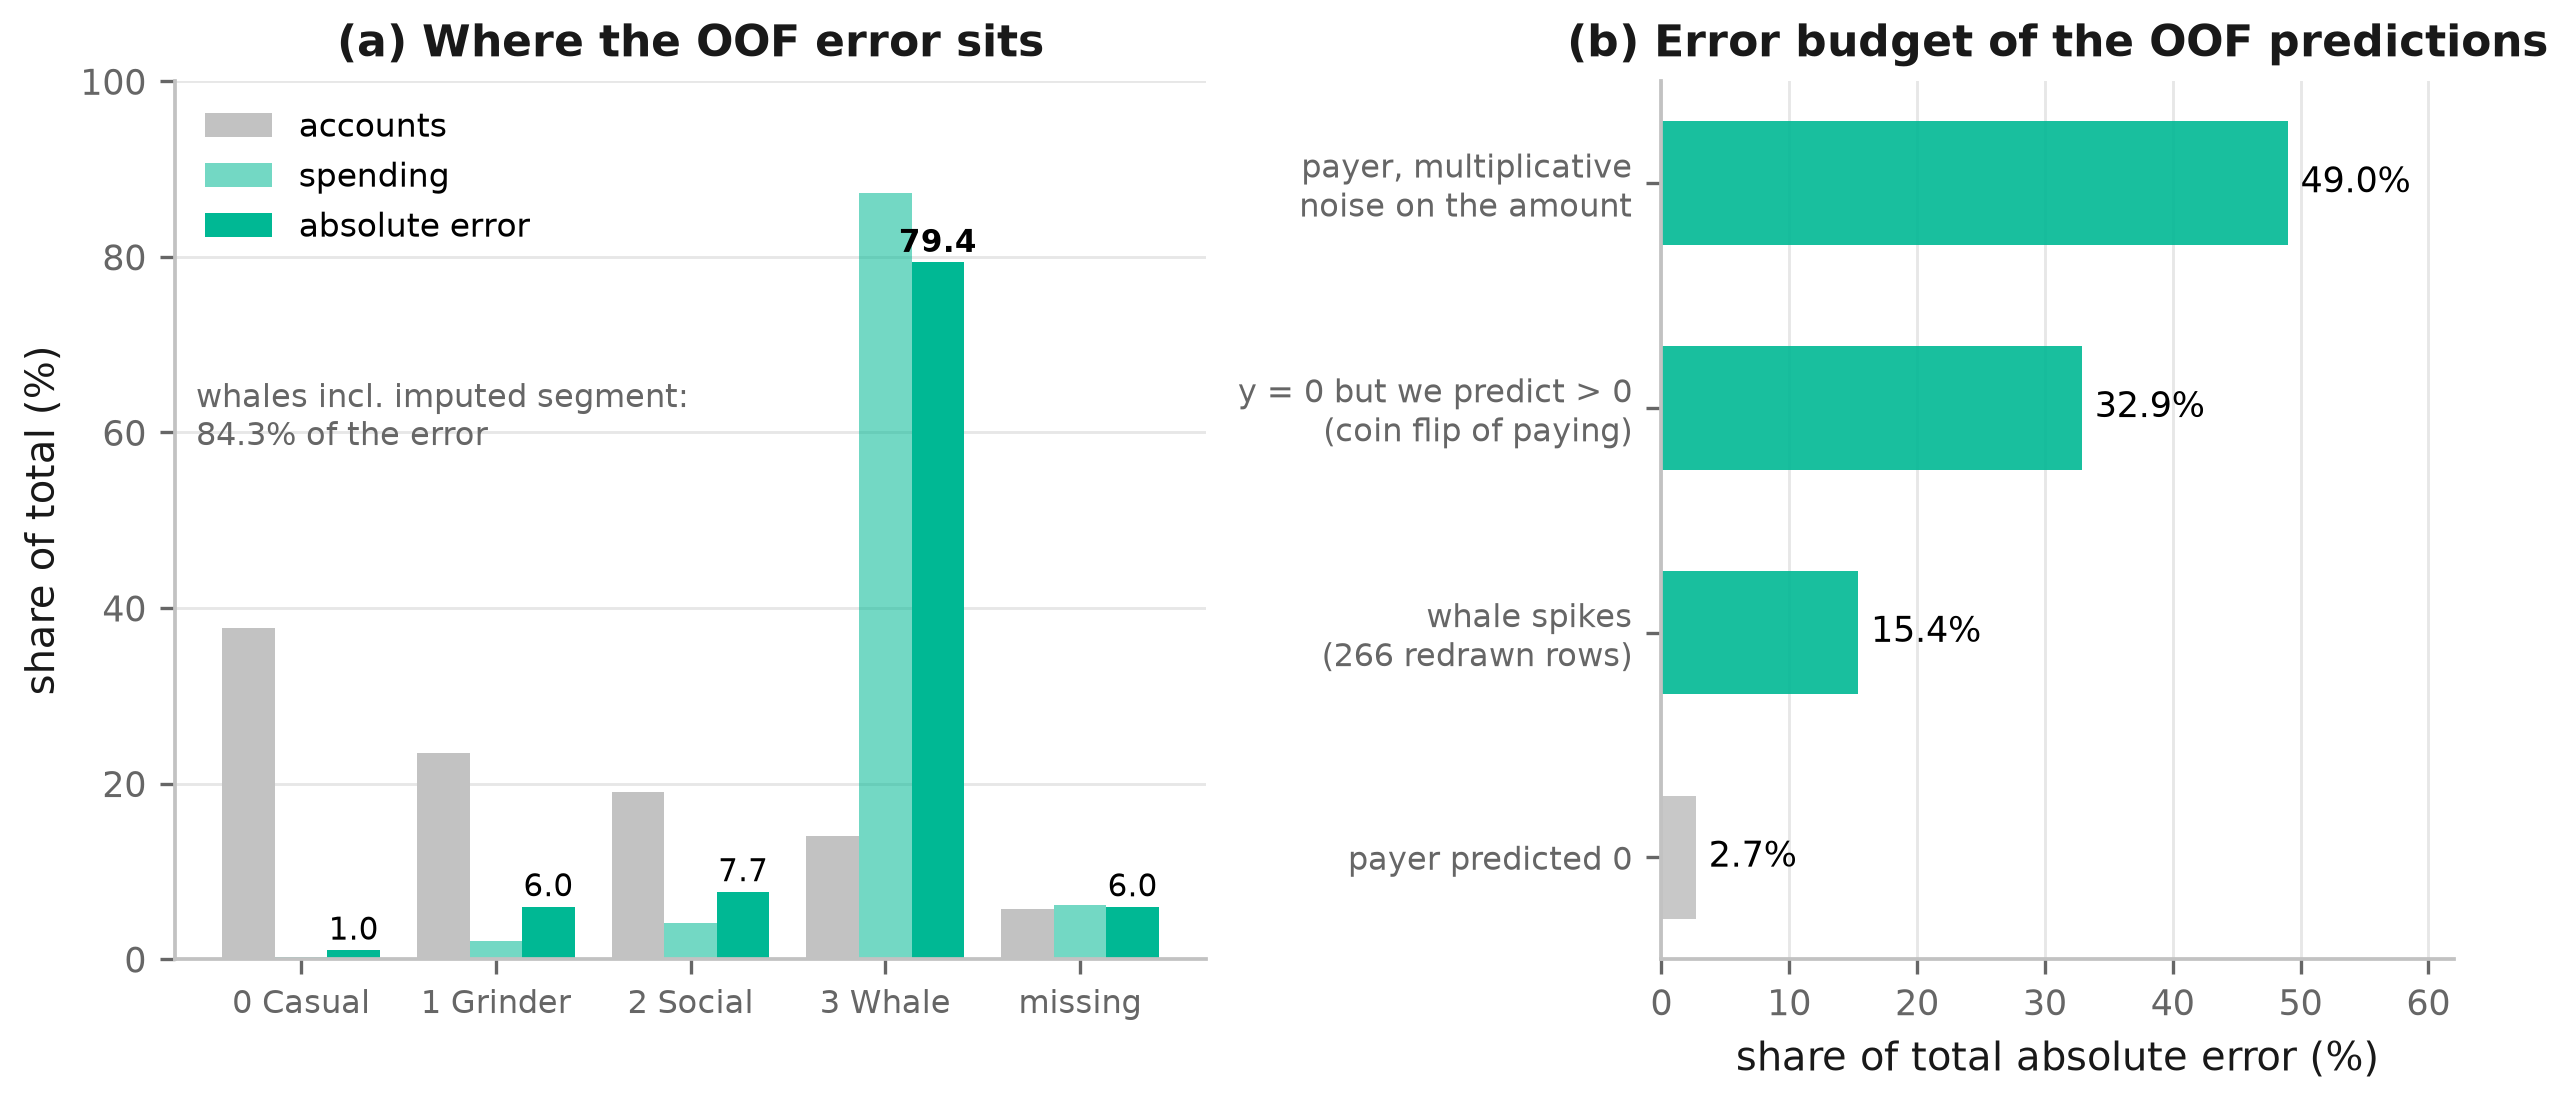
\includegraphics[width=\linewidth,height=0.33\textheight,keepaspectratio]{fig_t3_error_budget.png}
\caption{(a) Shares of accounts, spending and absolute error by segment. (b) The four sources of the total absolute error: multiplicative noise among payers, zero-spenders that are predicted as payers, 266 whale spikes, and payers predicted as zero.}
\label{fig:t3-error}
\end{figure}

Whales hold 79.4\% of the absolute error when they are defined by the recorded segment (Figure~\ref{fig:t3-error}a, the 14.0\% of rows with segment 3). The rows without a segment carry another 6.0\%; when the segment imputer assigns them (14.9\% of rows are then whales, with 93.0\% of the spending), whales hold \textbf{84.3\%} of the error, of which 60.7\% comes from paying whales and 23.6\% from whales that did not pay. Both numbers are computed from the saved $10\times10$ bag OOF (NMAE 0.79537); the three-seed OOF \texttt{best\_oof.csv} (0.79529) gives the same 79.4\% and 84.3\%, and the research report's 84.3\% used the imputed segments. In relative terms they are the best predicted segment (error equals 23\% of their spending, against 99\% for Casual players; 0.234 by recorded segment, 0.233 with the imputed one), but their amounts are so large that they still dominate. Panel (b) shows that nearly all of the error is chance: 49.0\% is the multiplicative noise on a payer's amount, 32.9\% comes from players who did not pay although we predicted a payment (a coin flip that a probability of 0.6--0.9 cannot resolve), 15.4\% from 266 whales (1.7\% of whales) whose spending was drawn from a different range of 90{,}000--290{,}000 THB regardless of last month, and only 2.7\% from payers that we predicted as zero.

\paragraph{The data have a floor.} Without the 266 spike rows the same predictions would score 0.8135, and with every zero known in advance 0.8527. We found, in the training data, that the payer amount equals last month's spending times a base ratio for the segment (about 1.10, 1.63, 1.82 and 3.04) times a few step factors (premium about $\times1.52$, each additional VIP tier about $\times1.1$, each extra game $\times1.07$, the months 0 and 11 $\times1.26$, a purchase within 15 days $\times1.16$) times a bounded noise with a log-standard-deviation of 0.15 in every segment. The learning curve of that noise is flat (0.158 at 5{,}000 rows, 0.152 at 38{,}000). We read this as a floor of about 0.796 for this metric, and our score of 0.7954 sits at it.

\paragraph{Why the log-normal head lost to quantiles.} Figure~\ref{fig:t3-ziln} compares the neural ZILN with the final model on the same out-of-fold rows (the saved network predictions line up with the training rows exactly).

\begin{figure}[H]
\centering
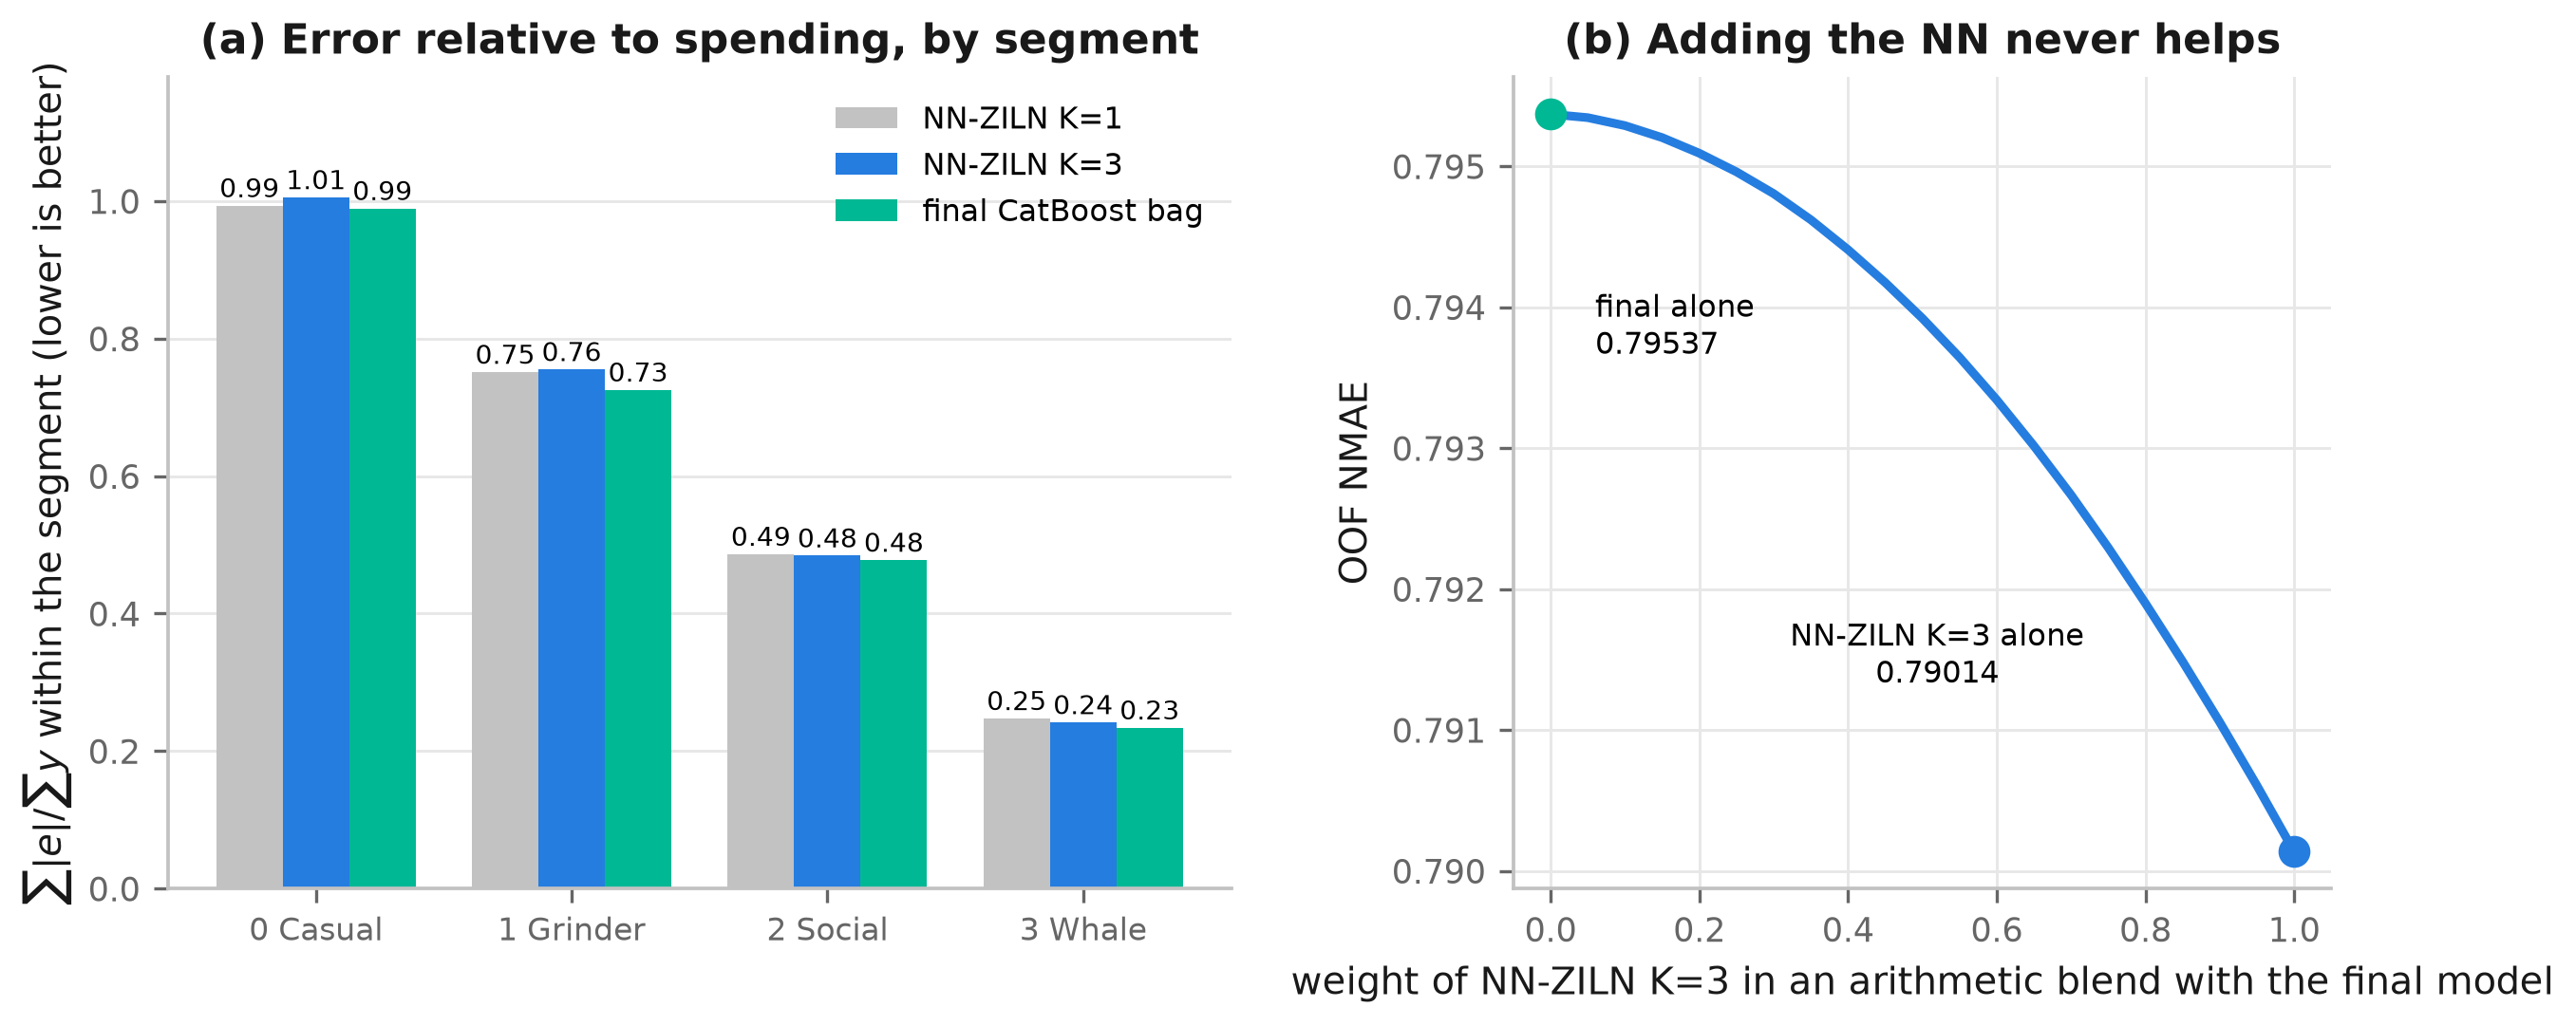
\includegraphics[width=\linewidth,height=0.33\textheight,keepaspectratio]{fig_t3_ziln_diag.png}
\caption{(a) Error relative to spending in each segment for the neural ZILN ($K=1$, $K=3$) and the final CatBoost bag. (b) OOF NMAE of an arithmetic blend of the final model with the $K=3$ network; no weight above zero improves the score.}
\label{fig:t3-ziln}
\end{figure}

\emph{What we see.} The final model has the lower error ratio in every segment, most clearly for Grinders (0.726 against 0.755 for $K=3$) and whales (0.234 against 0.242), and going from $K=1$ to $K=3$ already closes part of the gap (0.7867 to 0.7901). The XGBoost log-normal head of version 4 scores 0.7900 against 0.7917 for the multi-quantile model on the same features and probabilities, so a single parametric payer law costs about 0.0017 there. A log-normal has a heavy right tail and a smooth density, whereas the payer residual is a bounded noise with a log-standard-deviation of 0.15 plus a few spikes; the quantile we need is in the lower half of the distribution (Section~\ref{sec:t3-design}), where the shape of the tail should not matter, but a likelihood fit can still be pulled by the spikes (we did not test this separately). Adding the network does not help the final model: an arithmetic blend scores 0.79529 at weight 0.1 and 0.79392 at weight 0.5, against 0.79537 alone. \emph{What we decided.} Drop the ZILN branch from the final model.

\paragraph{Calibration and totals.} The model is calibrated where it matters. Predicted payer probabilities match observed rates in every bin (Figure~\ref{fig:t3-qrule}b). It predicts zero for 73\% of the true non-payers and for 29\% of the true payers, and the sum of its out-of-fold predictions is 100.2\% of the true total spending.

\paragraph{Ranking whales.} Ranking players by predicted spending puts 91.9\% of the true spending into the top 14\% (the best possible ranking gives 93.4\%), and 52.6\% into the top 5\% (best possible 58.4\%). Of the 5\% biggest true spenders, 84\% are also in the predicted top 5\%.

\subsubsection{Common Mistakes and Failed Experiments}
\label{sec:t3-mistakes}

\paragraph{Metric and objective.} We began with the assumption that the score is $1/(1+\mathrm{MAE}/\overline{|y|})$ and tested it with a probe in which Task~3 was set to zero for every player: the public score fell by 0.0590, exactly as predicted for a 0.795 model at a task weight of 0.2. Before that probe, predicting an expected value was one of our hypotheses; Table~\ref{tab:t3-rule} shows that an expected-value style rule loses 0.0086. The two-stage structure had been the hint in the brief (``will they spend, and how much'') and the quantile rule makes it exact for MAE.

\paragraph{Experiments that did not help.} Table~\ref{tab:t3-failed} lists them. The recurring lesson is that once the hurdle, the offset and the shallow quantile model are in place, every idea we tried changed the score by less than the standard deviation across folds (0.0076) or only by noise on the third digit.

\begin{table}[H]\centering\small
\caption{Task 3 experiments that were not adopted (OOF NMAE change relative to the model they were added to).}\label{tab:t3-failed}
\begin{tabular}{@{}L{.38\linewidth}L{.16\linewidth}L{.38\linewidth}@{}}
\toprule
\textbf{Experiment} & \textbf{Change} & \textbf{Reading} \\
\midrule
Direct log-link MAE on raw $y$ & $-0.0146$ & Stops early and cannot reach exact zeros. \\
Whale-only specialist & $-0.0026$ & Loses information shared across segments. \\
Fitted linear or ridge offset instead of unit slope & $-0.0012$ to $-0.0018$ & Whale spikes bias the fitted slope. \\
Sample weights proportional to $\sqrt{\text{prev}}$ & $-0.0014$ & Breaks the calibration of the pinball loss. \\
Purchase-cadence features & $-0.00023$ & Paired CV, 4 of 5 folds worse. \\
Fourier month features & $-0.00009$ & Paired CV, 5 of 5 folds worse. \\
Optuna search on CatBoost & $-0.00013$ & Gain on folds 0--1 vanished on folds 2--4. \\
Fill of \feat{is_premium_member} from the identity \feat{vip_status}$\ge3$ & $-0.00007$ & Exact identity, but CatBoost already reads it from VIP tier. \\
Pooled residual-quantile shape instead of 11 fitted quantiles & $-0.00007$ & The noise has one shape for every payer. \\
Native categoricals in CatBoost & $+0.00007\pm0.00011$ & 3 of 5 folds: noise. \\
Neural ZILN, mixture of 3 log-normals (alone 0.7901), blended into the final model & 0 (our log); $-0.0001$ at weight 0.1 in a plain blend (Figure~\ref{fig:t3-ziln}) & No gain on top of the CatBoost quantile model; it had helped the XGBoost stack (0.7920 to 0.7925). \\
Drop the worst 1/3/5/10\% residual rows, or Cauchy weights (R7) & $-0.00001$ to $-0.00031$; Cauchy $-0.00018$ & Paired CV. The noise is near-Gaussian and homogeneous (robust sd 0.17, 99th percentile 0.43), so there are no bad labels to remove. \\
IsolationForest or Mahalanobis drop of payers, 8 PCA features, 13-feature model (R8) & $+0.00013$ (best) to $-0.00024$ & Paired CV; the best case is not monotone in the drop rate. Unusual payers are real players; 36 of 49 features are ignored anyway (13 features: $+0.00008\pm0.00039$). \\
Nested LAD stack of 12 bases, Caruana greedy selection, family-equal blend, geometric against arithmetic mean (R5, E27) & $-0.00003$ to $-0.00006$ & Weights are unstable across folds; all within $\pm0.0001$ (Figure~\ref{fig:t3-paired}). \\
Post-hoc (shift, kappa) calibration, seven variants (R3) & $-0.00001$ to $+0.00001$ & Already calibrated (Section~\ref{sec:t3-eval}). \\
$50/50$ robust blend with a second quantile model & 0 (public) & Public score identical to the single model. \\
\bottomrule
\end{tabular}
\end{table}

\paragraph{Noise, outliers and ensemble selection.} After the final model was fixed we spent two rounds on the target noise and one on ensembling, all as paired out-of-fold comparisons on the same folds (Figure~\ref{fig:t3-paired}; the shaded band is the 0.0005 noise bar we used). Optuna \citep{optuna} tuning of CatBoost belongs to the same family and is in Table~\ref{tab:t3-failed}.

\begin{figure}[H]
\centering
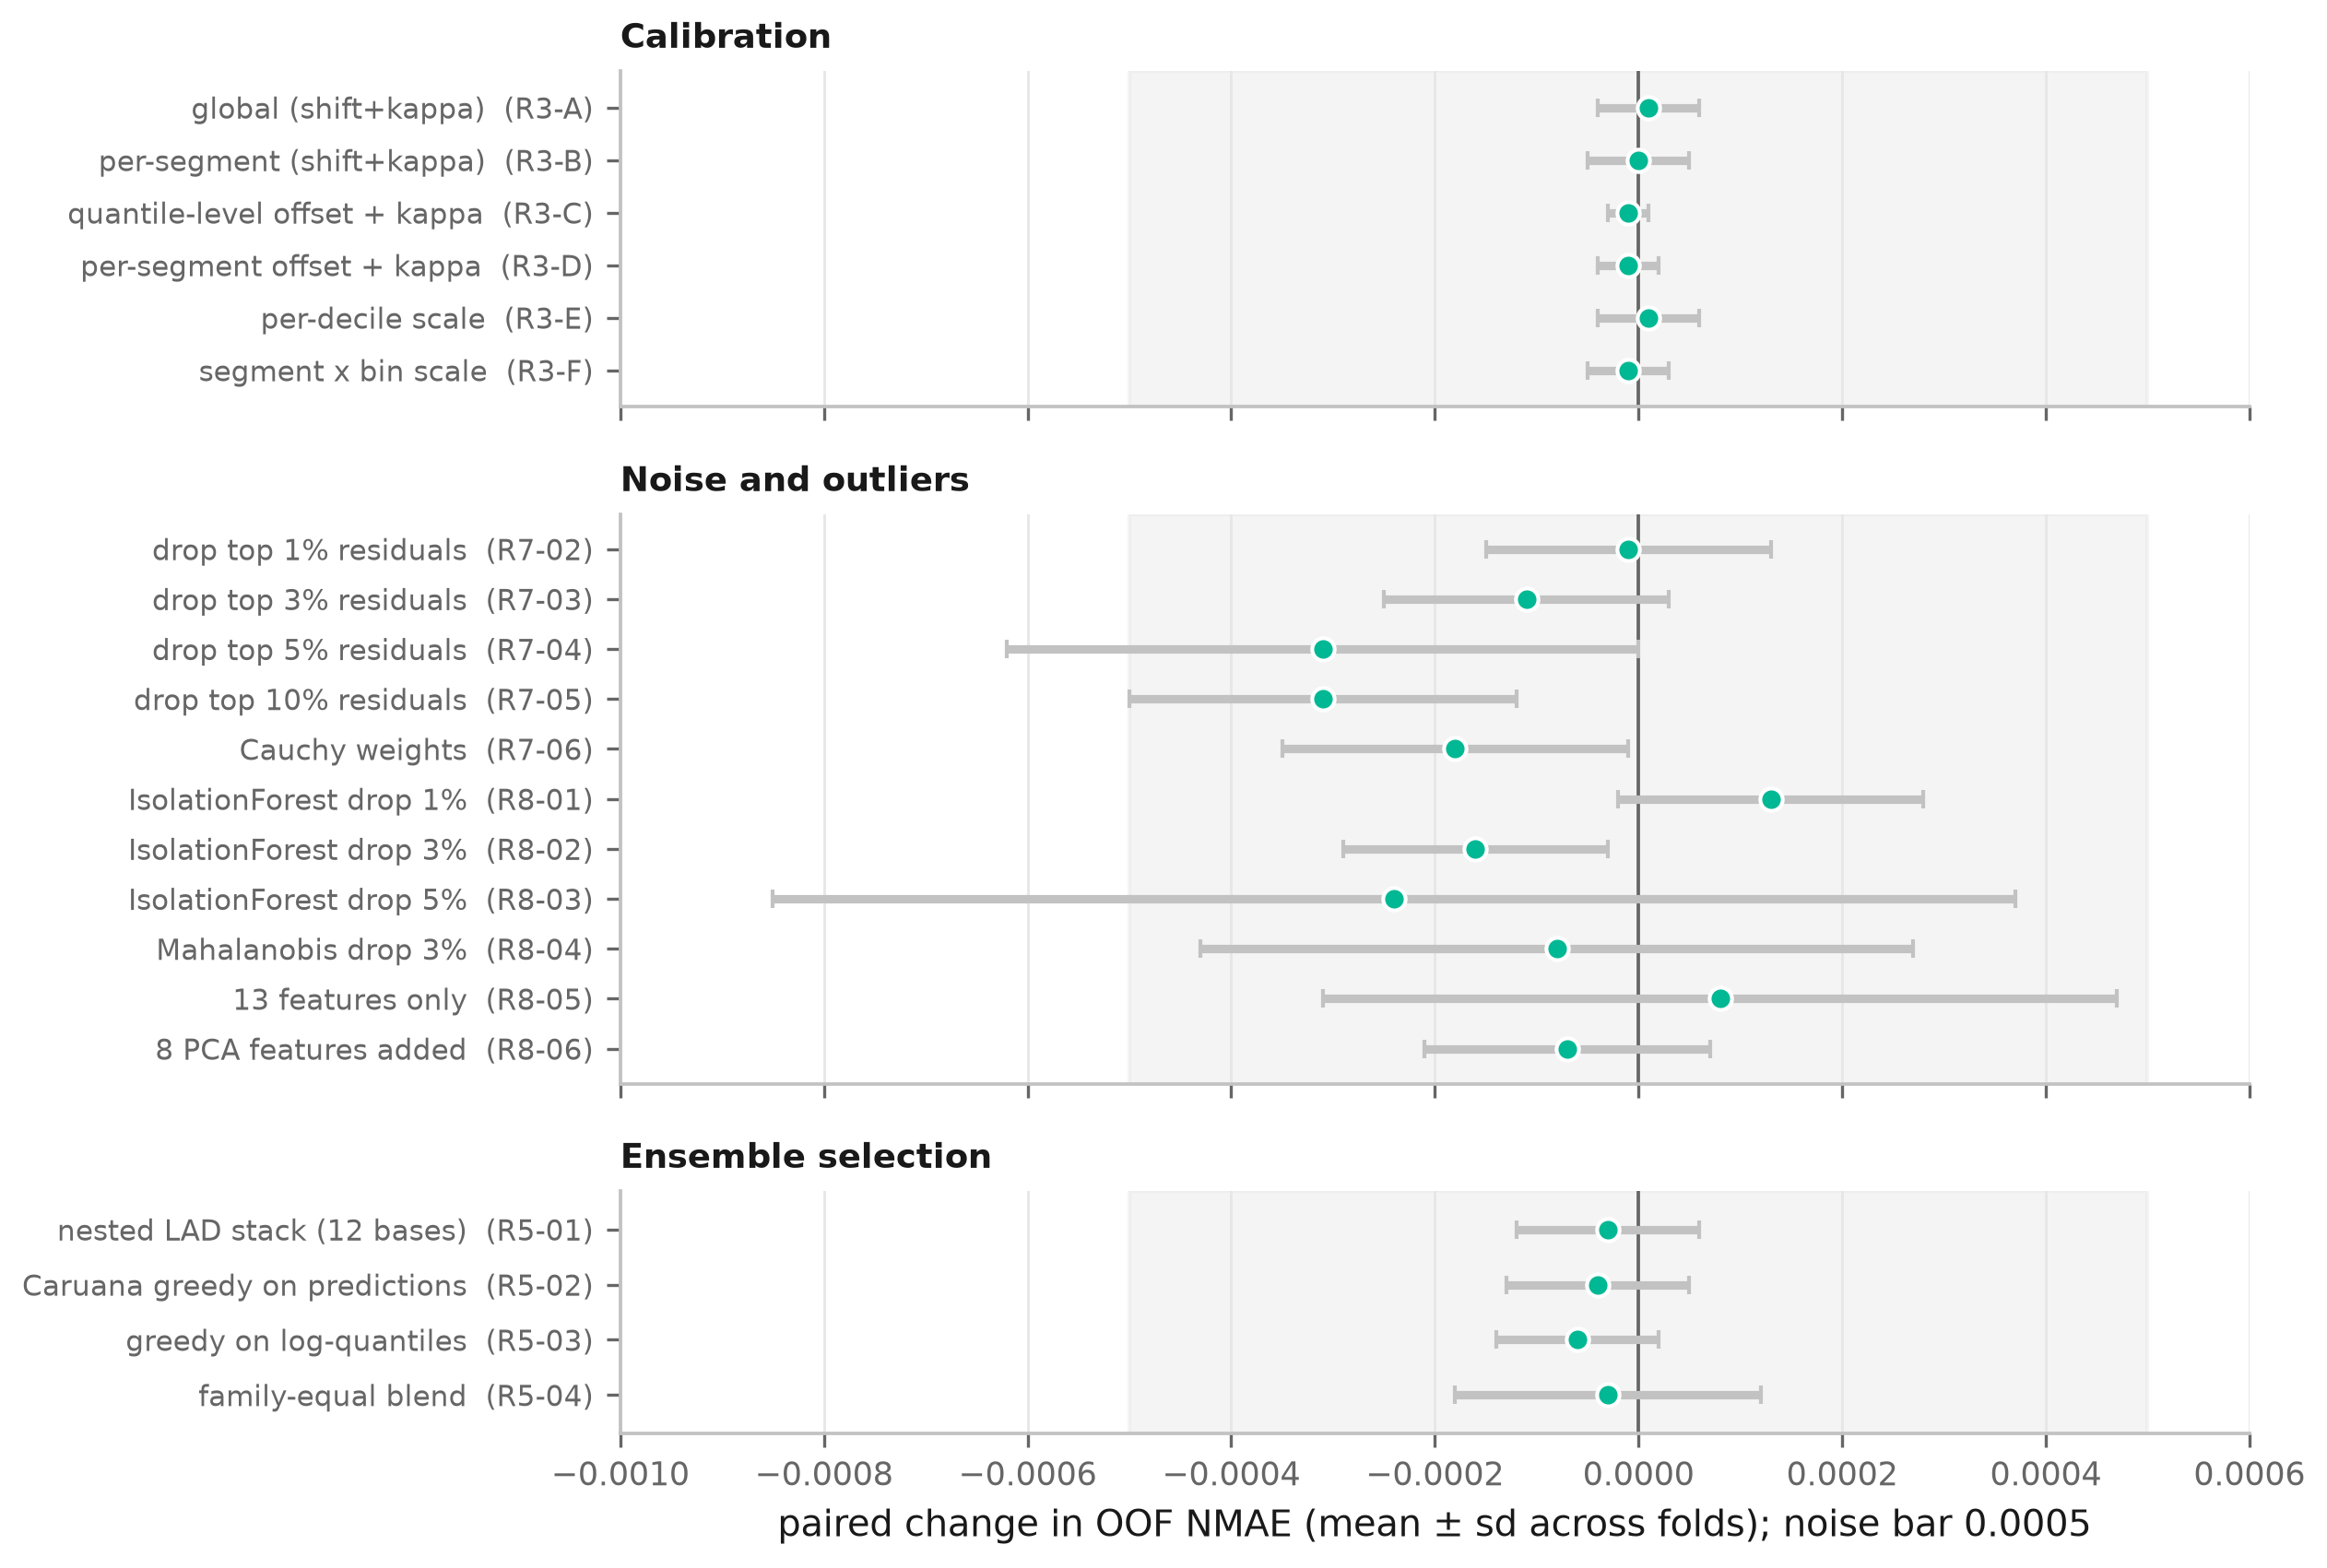
\includegraphics[width=.92\linewidth,height=0.46\textheight,keepaspectratio]{fig_t3_paired.png}
\caption{Paired change in OOF NMAE (mean and standard deviation over the five folds) for post-hoc calibration, noise and outlier handling, and ensemble selection. Calibration and ensemble rows are measured against the final $3\times3$ bag (0.79529); noise rows against a same-code control (0.79512). No row clears the noise bar.}
\label{fig:t3-paired}
\end{figure}

\emph{Noise.} The residuals of the training payers are near-Gaussian and homogeneous (robust standard deviation 0.17 in log, 99th percentile 0.43, only about 0.65\% beyond four standard deviations; R7-00), so there is no separable group of bad labels. Dropping the largest 1, 3, 5 or 10\% of residuals (inside each training fold only; validation folds untouched) or down-weighting them with a Cauchy weight changes the score by $-0.00001$, $-0.00011$, $-0.00031$, $-0.00031$ and $-0.00018$: monotonically worse, because the quantile we need (about 0.46) lives in the tail that the dropped rows carry. Without the target, an Isolation Forest \citep{isolationforest} drop of 1\% scored $+0.00013\pm0.00015$, but 3\% and 5\% scored $-0.00016$ and $-0.00024$; a Mahalanobis drop of 3\% in PCA space scored $-0.00008$, eight PCA components as features $-0.00007$, and a model on the 13 features with non-negligible importance $+0.00008\pm0.00039$ (36 of 49 features have importance below 0.5\%, but the trees already ignore them). \emph{Decision.} Train on all rows with all features.

\emph{Ensemble selection.} With twelve base models (CatBoost depths 3, 4, 6 and 8, XGBoost, LightGBM and a from-scratch network written in PyTorch \citep{pytorch}), a nested LAD stack scored $-0.00003$ against the untuned final bag (R5-01; at an earlier stage, on the XGBoost model, the same kind of stack gained $+0.00016$, E11), Caruana greedy selection \citep{caruana} on the predictions $-0.00004$ and on the log-quantiles $-0.00006$ (R5-02, R5-03), and the weights moved by up to 0.09 between folds. A family-equal blend (CatBoost depths 3, 4, 6 and XGBoost depth 5, a quarter each) scored $-0.00003\pm0.00015$ and has the best worst-fold score (0.78336 against 0.78328); we keep it as a robust alternative file, which differs from the final test predictions by 0.6\% on average (correlation 0.99997). Averaging the hurdle predictions of six models instead of their quantiles also changed nothing ($-0.00006$, E27). \emph{Decision.} Equal-weight seed bag of one family, no tuned weights.

\paragraph{The ZILN detour.} We spent the first stage of Task~3 on ZILN because it is the textbook loss for a zero-inflated, positive and multiplicative target, and it did give a strong baseline (0.7893 to 0.7925 across five stages and a neural variant). Two things we would do differently. First, the metric needs one quantile of the payer distribution (from the start we used $q=1-1/(2p)$ on top of ZILN), so a loss that fits the whole shape adds a parametric assumption that the metric does not need; the pinball loss on 11 quantiles fits what is read off directly. Second, we tuned the ZILN stages on the same out-of-fold rows we scored them on (the 0.7920 and 0.7925 weights are in-sample; the nested value of the XGBoost blend is 0.79191), so part of their lead over HGB was optimistic. The CatBoost model has no tuned weights, so its 0.79535 needs no such correction. When the quantile model arrived, the NN no longer added anything, and the ZILN code was left in the repository as notebooks \texttt{task3-hurdle-ziln}, \texttt{task3-hurdle-ziln-v4} and \texttt{task3-nn-ziln}.

\paragraph{Rule compliance.} Task~3 involved no leak and no test statistic. The segment imputer, the exact fill, the folds and every threshold are computed from training rows, and the clip value of 300{,}000 is the maximum of the training target. A teammate's variant on the re-released data that mixed a Jensen correction with a hard zero cut-off scored 0.00011 below the model it modified on the public leaderboard, and we did not adopt it.

\paragraph{A correction to our own EDA.} An early note in our EDA said that the log-residual is ``centred''. The histogram in Figure~\ref{fig:t3-offset}b shows that it is tight but \emph{shifted by segment}; the model does not need it to be centred, but the statement was wrong.

\subsubsection{Domain Interpretation and Business Impact}

Karena's finance team misses quarterly targets by 35--40\%, the 20-person VIP support team does not know whom to prioritise, and discount codes go to whales who would have paid anyway (more than 6 million baht a month, according to the brief). The model speaks to each of these in a different way.

\paragraph{Prioritising VIP support.} Ranking players by predicted spending puts 91.9\% of the true spending into the top 14\% of players, and 52.6\% into the top 5\% (Section~\ref{sec:t3-eval}). A team of 20 can concentrate its time on that group. In the brief's example, a whale who spent 255{,}000 baht waited three days while the team served 150 players with high playtime who spent 12{,}000 baht together; a list ranked by this model would have placed the whale at the top.

\paragraph{Targeted offers.} The payer probability $p$ separates two actions. A player with high $p$ and high predicted spending needs a fast, personal service and no discount. A player with $p$ near 0.5 is the one where an offer can still change the decision. Because $p$ is calibrated, a marketing team can set a budget on expected conversions.

\paragraph{Revenue forecasting.} The out-of-fold predictions add up to 100.2\% of the real total, so a portfolio total for a month is close even though each prediction is a median. A median forecast is not an unbiased forecast in general, so this agreement should not be relied on; a finance team should also keep the 11 quantiles, which describe the spread of the lower half, and calibrate the totals on the last closed quarter before using them in a budget.

\paragraph{Limits.} The score of 0.795 is a floor set by the generator; on live data we would expect different noise. About a third of the error is unpredictable coin-flips on whether a player pays, so no individual prediction should be presented as a promise. The 266 whale spikes show that a few large, unforeseen purchases dominate any monthly total; finance should add a reserve for them instead of expecting a model to find them.

\end{document}
